\documentclass{article}
\usepackage[T1]{fontenc}
\usepackage{lmodern}
\usepackage{graphicx}
\usepackage{amsmath,amssymb}
\usepackage[a4paper,margin=2cm]{geometry}
\usepackage[absolute,overlay]{textpos}
\setlength{\TPHorizModule}{1mm}
\setlength{\TPVertModule}{1mm}
\usepackage[indonesian]{babel}
\usepackage{hyperref}
\setlength{\emergencystretch}{2em}
\title{10-Beberapa-block-cipher-bagian2-2026}
\author{pdf\_ppt\_to\_latex}
\date{}

\begin{document}

% --- unit llm 1 ---
% === Halaman 1 (llm) ===

\begin{center}
Bahan kuliah IF4020 Kriptografi

{\huge \color{red} 10- Review Beberapa Block Cipher}
{\large \color{red} (Bagian 2: Advanced Encryption Standrad - AES)}

\vspace{30mm}

Oleh: Rinaldi M

\vspace{10mm}

Program Studi Teknik Informatika\\
Sekolah Teknik Elektro dan Informatika\\
Institut Teknologi Bandung\\
2026
\end{center}

\newpage

% --- unit llm 2 ---
% === Halaman 2 (llm) ===

\section*{Latar Belakang}

\begin{itemize}
    \item DES dianggap sudah tidak aman karena kunci dapat ditemukan secara \textit{brute-force}.
    \item Perlu diusulkan standard algoritma baru sebagai pengganti DES.
    \item \textit{National Institute of Standards and Technology} (NIST) mengusulkan kepada Pemerintah Federal AS untuk sebuah standard kriptografi baru.
    \item NIST mengadakan kompetisi terbuka untuk membuat standard algoritma kriptografi yang baru. Standard tersebut kelak diberi nama \textbf{Advanced Encryption Standard (AES)}.
\end{itemize}

\newpage

% --- unit llm 3 ---
% === Halaman 3 (llm) ===

Persyaratan AES:\
\begin{enumerate}
  \item Termasuk ke dalam kelompok algoritma kriptografi simetri berbasis \textit{cipher} blok.
  \item Seluruh rancangan algoritma harus publik (tidak dirahasiakan, tidak ada yang disembunyikan)
  \item Panjang kunci fleksibel: 128, 192, dan 256 bit.
  \item Ukuran blok yang dienkripsi adalah 128 bit.
  \item Algoritma dapat diimplementasikan baik sebagai \textit{software} maupun \textit{hardware}.
\end{enumerate}

\newpage

% --- unit llm 4 ---
% === Halaman 4 (llm) ===

Lima finalis lomba AES:
\begin{enumerate}
  \item \textit{Rijndael} (dari Vincent \textbf{Rijmen dan} Joan \textbf{Daemen} -- Belgia, 86 suara)
  \item \textit{Serpent} (dari Ross Anderson, Eli Biham, dan Lars Knudsen -- Inggris, Israel, dan Norwegia, 59 suara).
  \item \textit{Twofish} (dari tim yang diketuai oleh Bruce Schneier -- USA, 31 suara)
  \item \textit{RC6} (dari Laboratorium RSA -- USA, 23 suara)
  \item \textit{MARS} (dari IBM, 13 suara)
\end{enumerate}

\newpage

% --- unit llm 5 ---
% === Halaman 5 (llm) ===

\begin{itemize}
  \item Pada bulan Oktober 2000, \textit{NIST} mengumumkan untuk memilih Rijndael (dibaca: Rhine-doll)
  \item Pada bulan November 2001, Rijndael ditetapkan sebagai AES
\end{itemize}

\vspace{50mm}

\begin{itemize}
  \item Diharapkan Rijndael menjadi standard kriptografi yang dominan paling sedikit selama 10 tahun.
\end{itemize}

% deskripsi: Foto dua orang pria di depan papan bertuliskan AES (Advanced Encryption Standard)
% bbox normalisasi: [0.2710, 0.3380, 0.6080, 0.7630]
\begin{textblock*}{70.77mm}(56.91mm,100.39mm)
\noindent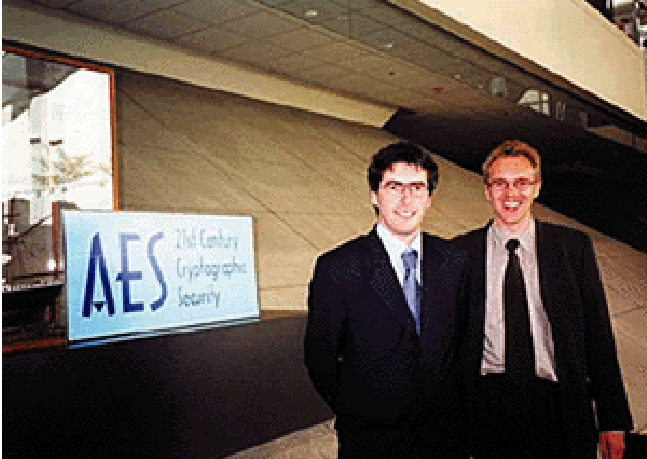
\includegraphics[width=70.77mm,height=126.22mm]{images/llm/page_005_img_01.png}%
\end{textblock*}

\newpage

% --- unit llm 6 ---
% === Halaman 6 (llm) ===

\vspace{192.46mm}

Joan Daemen and Vincent Rijmen, the designers of the Advanced Encryption Standard
(Sumber: \url{https://medium.com/@stkgroup/what-is-the-advanced-encryption-standard-and-how-does-it-work-abd1ec582df8})

% deskripsi: Foto Joan Daemen dan Vincent Rijmen, perancang Advanced Encryption Standard (AES).
% bbox normalisasi: [0.1970, 0.0540, 0.7650, 0.7020]
\begin{textblock*}{119.28mm}(41.37mm,16.04mm)
\noindent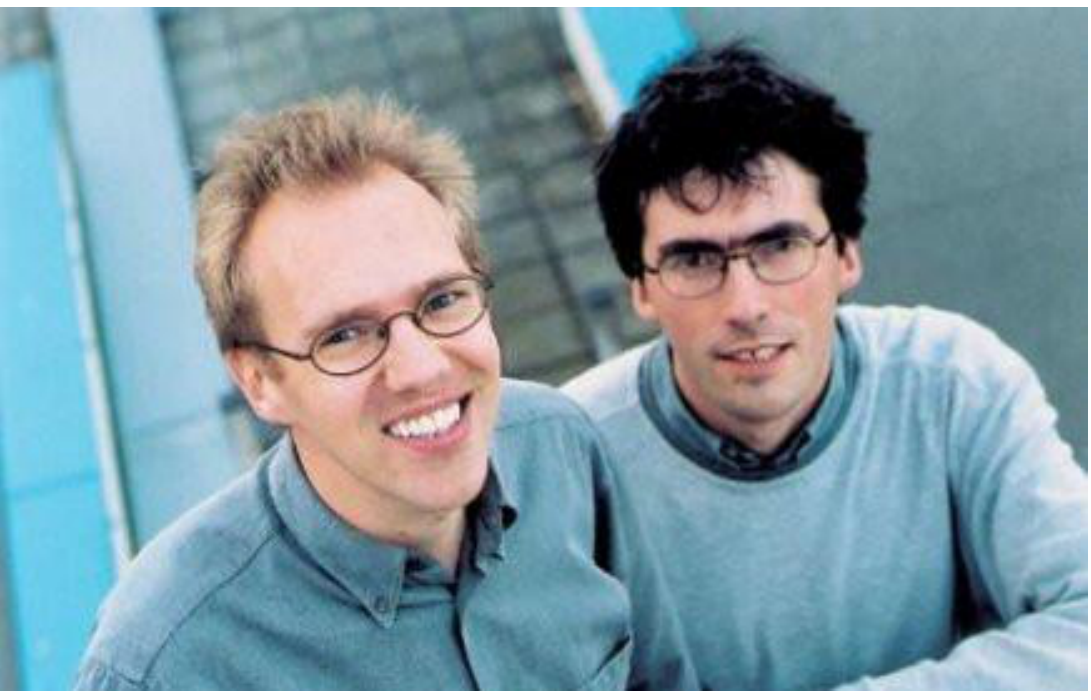
\includegraphics[width=119.28mm,height=192.46mm]{images/llm/page_006_img_01.png}%
\end{textblock*}

\newpage

% --- unit llm 7 ---
% === Halaman 7 (llm) ===

\section*{Spesifikasi Algoritma Rijndael}

\begin{itemize}
    \item Rijndael mendukung panjang kunci 128 bit sampai 256 bit dengan step 32 bit (yaitu 128 bit, 160, 192, ..., 256 bit).
    \item Panjang kunci dan ukuran blok dapat dipilih secara independent (tidak harus sama. Misal: panang blok 128 bit, kunci 256 bit).
    \item Setiap blok dienkripsi dalam sejumlah putaran tertentu, sebagaimana halnya pada $DES$.
    \item Karena $AES$ menetapkan panjang kunci adalah 128, 192, dan 256, maka dikenal AES-128, AES-192, dan AES-256.
\end{itemize}

\newpage

% --- unit llm 8 ---
% === Halaman 8 (llm) ===

\vspace{20mm}

Catatan: 1 $word = 32$ bit

\begin{itemize}
    \item Secara de-fakto, hanya ada dua varian $AES$, yaitu $AES$-128 dan $AES$-256, karena akan sangat jarang pengguna menggunakan kunci yang panjangnya 192 bit.
\end{itemize}

% deskripsi: Tabel parameter AES yang menunjukkan Panjang Kunci (Nk words), Ukuran Blok (Nb words), dan Jumlah Putaran (Nr) untuk varian AES-128, AES-192, dan AES-256.
% bbox normalisasi: [0.2840, 0.1940, 0.9060, 0.4300]
\begin{textblock*}{130.62mm}(59.64mm,57.62mm)
\noindent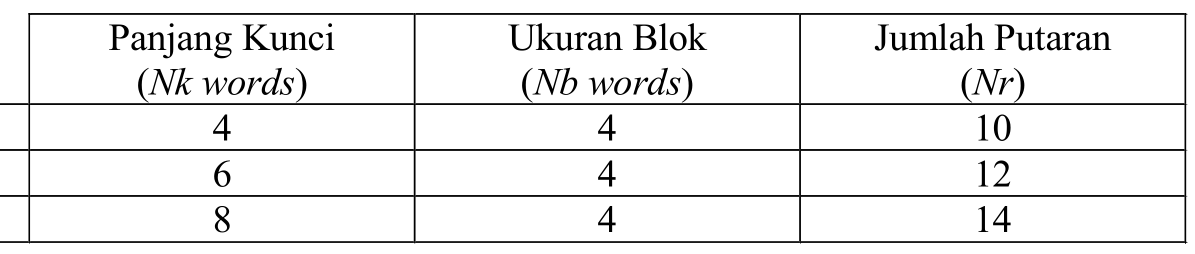
\includegraphics[width=130.62mm,height=70.09mm]{images/llm/page_008_img_01.png}%
\end{textblock*}

\newpage

% --- unit llm 9 ---
% === Halaman 9 (llm) ===

\begin{itemize}
    \item Dengan panjang kunci 128-bit, maka terdapat sebanyak
    \[ 2^{128} = 3,4 \times 10^{38} \text{ kemungkinan kunci.} \]
    \item Jika komputer tercepat dapat mencoba 1 juta kunci setiap detik, maka akan dibutuhkan waktu $5,4 \times 10^{24}$ tahun untuk mencoba seluruh kunci.
    \item Jika komputer tercepat yang dapat mencoba 1 juta kunci setiap milidetik, maka dibutuhkan waktu $5,4 \times 10^{18}$ tahun untuk mencoba seluruh kunci.
    \item Artinya, AES diharapkan tahan terhadap serangan \textit{exhaustive key search attack (brute force attack)}
\end{itemize}

\newpage

% --- unit llm 10 ---
% === Halaman 10 (llm) ===

\section*{Algoritma \textit{Rijndael}}

\begin{itemize}
    \item Yang dijelaskan di sini Rijndael 128-bit (anjang kunci 128 bit)
    \item Tidak seperti \textit{DES} yang berorientasi bit, \textit{Rijndael} beroperasi dalam orientasi \textit{byte}.
    \item \textit{Rijndael} tidak menggunakan jaringan Feistel seperti cipher blok lainnya.
    \item \textit{Enciphering} dilakukan dalam sejumlah putaran (iterate cipher). Setiap putaran mengunakan kunci internal yang berbeda (disebut \textit{round key}).
    \item \textit{Enciphering} melibatkan operasi substitusi dan permutasi.
\end{itemize}

\newpage

% --- unit llm 11 ---
% === Halaman 11 (llm) ===

\begin{itemize}
    \item Garis besar Algoritma \textit{Rijndael} yang beroperasi pada blok 128-bit dengan kunci 128-bit adalah sebagai berikut (di luar proses pembangkitan \textit{round key}):
    \begin{enumerate}
        \item \textit{AddRoundKey}: melakukan XOR antara \textit{state} awal (plainteks) dengan \textit{cipher key}. Tahap ini disebut juga \textit{initial round}.
        \item Putaran sebanyak $Nr - 1$ kali. Proses yang dilakukan pada setiap putaran adalah:
        \begin{enumerate}
            \item \textit{SubBytes}: substitusi \textit{byte} dengan menggunakan tabel substitusi (S-box).
            \item \textit{ShiftRows}: pergeseran baris-baris \textit{array state} secara \textit{wrapping}.
            \item \textit{MixColumns}: mengacak data di masing-masing kolom \textit{array state}.
            \item \textit{AddRoundKey}: melakukan XOR antara \textit{state} sekarang \textit{round key}.
        \end{enumerate}
        \item \textit{Final round}: proses untuk putaran terakhir:
        \begin{enumerate}
            \item \textit{SubBytes}
            \item \textit{ShiftRows}
            \item \textit{AddRoundKey}
        \end{enumerate}
    \end{enumerate}
\end{itemize}

\newpage

% --- unit llm 12 ---
% === Halaman 12 (llm) ===

\vspace{163.35mm}

Round key 0 \vspace{5mm} putaran awal \vspace{5mm} $Nr - 1$ putaran \vspace{5mm} Round key $Nr - 1$ \vspace{5mm} putaran akhir

% deskripsi: Diagram alir proses enkripsi AES (Advanced Encryption Standard) yang menunjukkan tahapan State, AddRoundKey, SubBytes, ShiftRows, MixColumns, dan penggunaan Round Key dari putaran awal hingga putaran akhir.
% bbox normalisasi: [0.2500, 0.3300, 0.5500, 0.8800]
\begin{textblock*}{63.00mm}(52.50mm,98.01mm)
\noindent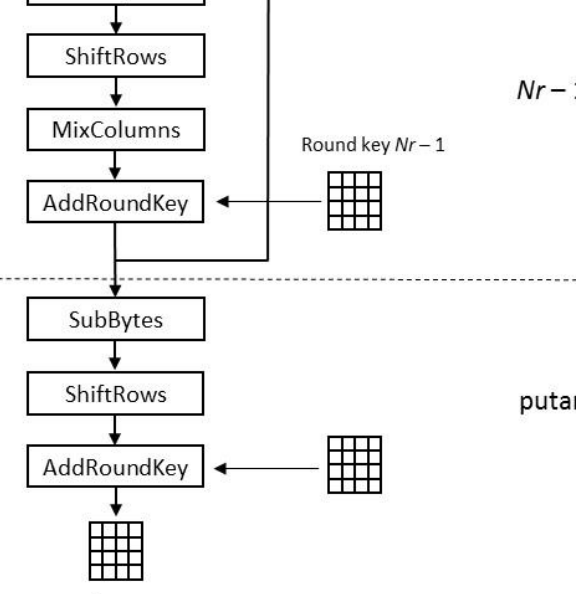
\includegraphics[width=63.00mm,height=163.35mm]{images/llm/page_012_img_01.png}%
\end{textblock*}

\newpage

% --- unit llm 13 ---
% === Halaman 13 (llm) ===

\vspace{237.60mm}

\textcolor{red}{Sumber: H\\u00e5kon Jacobsen, Lecture 2 -- Block ciphers, PRFs/PRPs, DES, AES}

\section*{AES-128}

\vspace{60mm}

% deskripsi: Diagram alur proses enkripsi AES-128 yang menunjukkan proses ekspansi kunci dari kunci utama K menjadi kunci putaran K0 hingga K10, serta struktur 10 putaran yang terdiri dari operasi SubBytes, ShiftRow, dan MixColumn.
% bbox normalisasi: [0.0150, 0.1400, 0.9850, 0.9400]
\begin{textblock*}{203.70mm}(3.15mm,41.58mm)
\noindent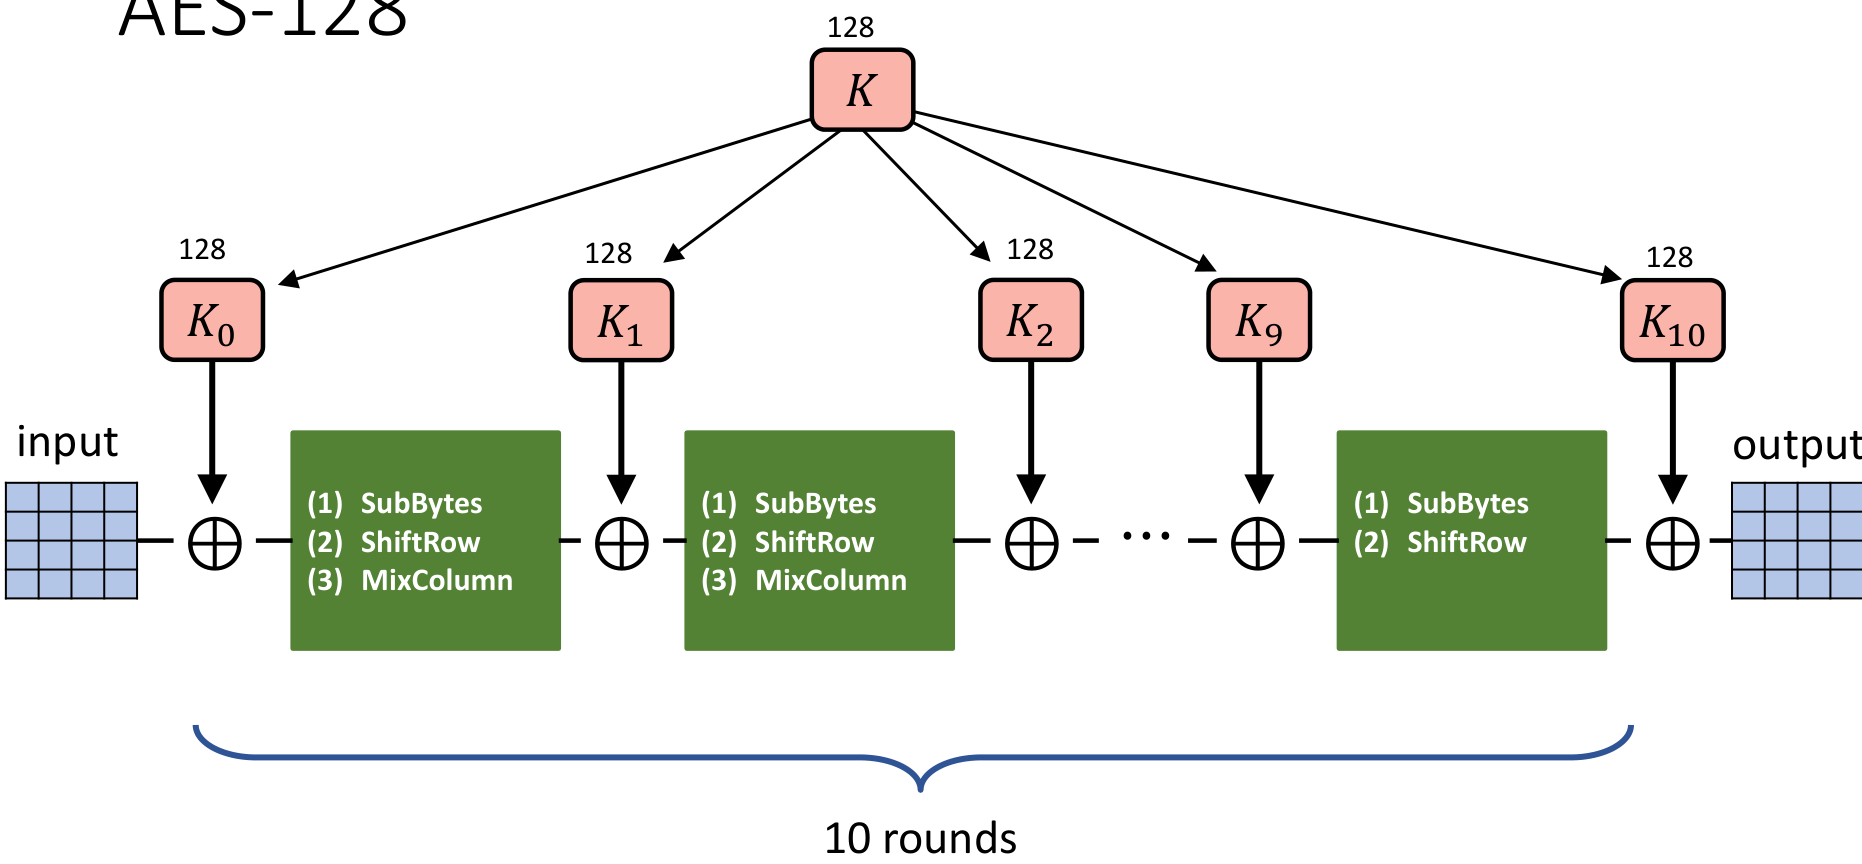
\includegraphics[width=203.70mm,height=237.60mm]{images/llm/page_013_img_01.png}%
\end{textblock*}

\newpage

% --- unit llm 14 ---
% === Halaman 14 (llm) ===

% (tidak ada teks dari model)

% deskripsi: Screenshot cuplikan kode program bahasa C untuk implementasi algoritma enkripsi Rijndael (AES).
% bbox normalisasi: [0.1100, 0.4000, 0.8410, 0.9110]
\begin{textblock*}{153.51mm}(23.10mm,118.80mm)
\noindent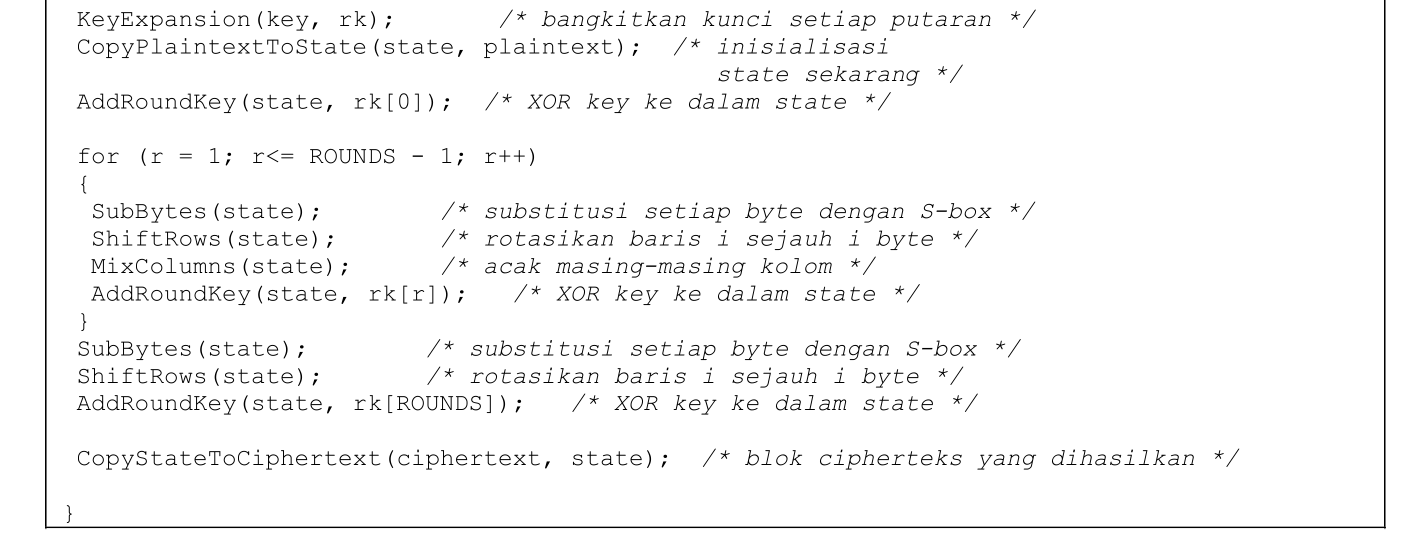
\includegraphics[width=153.51mm,height=151.77mm]{images/llm/page_014_img_01.png}%
\end{textblock*}

\newpage

% --- unit llm 15 ---
% === Halaman 15 (llm) ===

\vspace{205.23mm}

\begin{itemize}
    \item Selama kalkulasi plainteks menjadi cipherteks, status data sekarang disimpan di dalam matriks dua dimensi, \texttt{state}.
    \item \texttt{state} bertipe \textit{byte} dan berukuran $Nrows \times Ncols$
    \item Untuk blok data 128-bit, ukuran \texttt{state} adalah $4 \times 4$, seperti gambar di samping.
\end{itemize}

% deskripsi: Diagram yang menunjukkan transformasi plainteks 128-bit menjadi matriks state berukuran 4x4.
% bbox normalisasi: [0.6450, 0.1940, 0.8980, 0.8850]
\begin{textblock*}{53.13mm}(135.45mm,57.62mm)
\noindent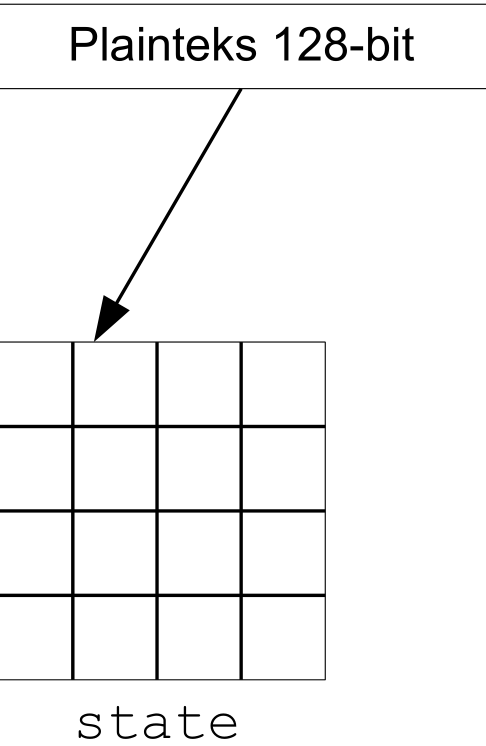
\includegraphics[width=53.13mm,height=205.23mm]{images/llm/page_015_img_01.png}%
\end{textblock*}

\newpage

% --- unit llm 16 ---
% === Halaman 16 (llm) ===

\begin{itemize}
    \item Pada awal enkripsi, 16-byte data masukan, $in_0, in_1, \dots, in_{15}$ disalin ke dalam array \texttt{state}, direalisasikan oleh fungsi:
    \[ \texttt{CopyPlaintextToState(state, plaintext)} \]
\end{itemize}

\vspace{60mm}

\begin{itemize}
    \item Pada akhir enkripsi, state disalin ke dalam \texttt{ciphertext}, direalisasikan oleh fungsi:
    \[ \texttt{CopyStateToCiphertext(ciphertext, state)} \]
\end{itemize}

% deskripsi: Diagram yang menunjukkan proses pemetaan data dari input bytes ke state array dan kemudian ke output bytes dalam bentuk matriks 4x4.
% bbox normalisasi: [0.1480, 0.2840, 0.8460, 0.6720]
\begin{textblock*}{146.58mm}(31.08mm,84.35mm)
\noindent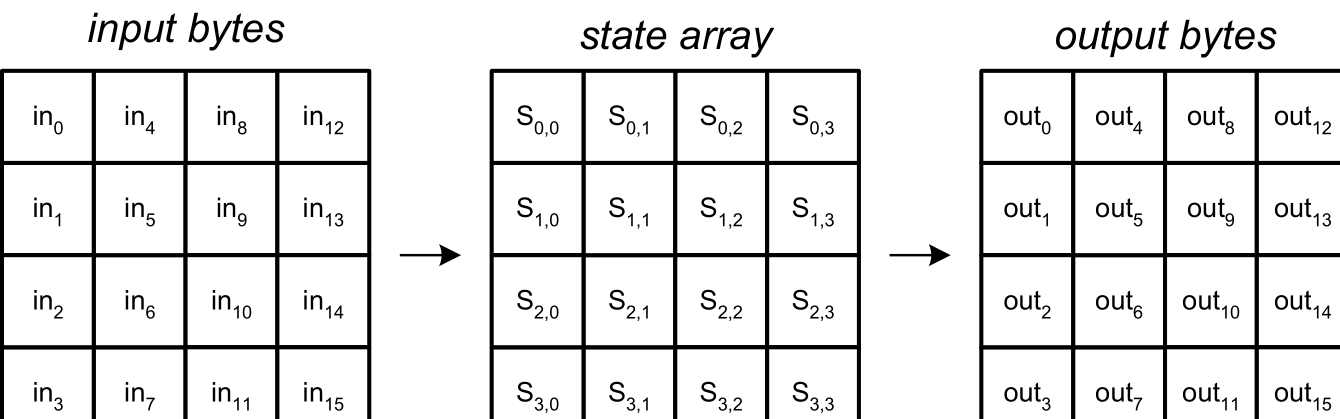
\includegraphics[width=146.58mm,height=115.24mm]{images/llm/page_016_img_01.png}%
\end{textblock*}

\newpage

% --- unit llm 17 ---
% === Halaman 17 (llm) ===

\vspace{100.68mm}

Contoh elemen state dalam notasi HEX:
\vspace{10mm}

% deskripsi: Tabel yang berisi elemen state dalam notasi heksadesimal (HEX) dengan ukuran 4x4.
% bbox normalisasi: [0.2460, 0.3270, 0.5350, 0.6660]
\begin{textblock*}{60.69mm}(51.66mm,97.12mm)
\noindent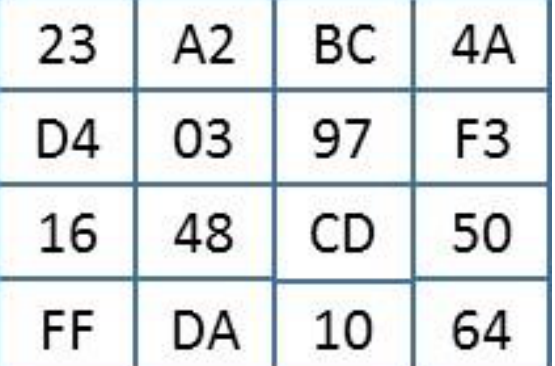
\includegraphics[width=60.69mm,height=100.68mm]{images/llm/page_017_img_01.png}%
\end{textblock*}

\newpage

% --- unit llm 18 ---
% === Halaman 18 (llm) ===

\section*{Transformasi $SubBytes()$}

\vspace{202.26mm}

\begin{itemize}
    \item $SubBytes()$ melakukan operasi substitusi dengan memetakan setiap byte dari array state dengan menggunakan S-box.
\end{itemize}

\vspace{10mm}

% deskripsi: Tabel S-box yang digunakan dalam transformasi SubBytes pada algoritma AES, berisi pemetaan nilai heksadesimal dari indeks baris dan kolom ke nilai substitusinya.
% bbox normalisasi: [0.2060, 0.2700, 0.7380, 0.9510]
\begin{textblock*}{111.72mm}(43.26mm,80.19mm)
\noindent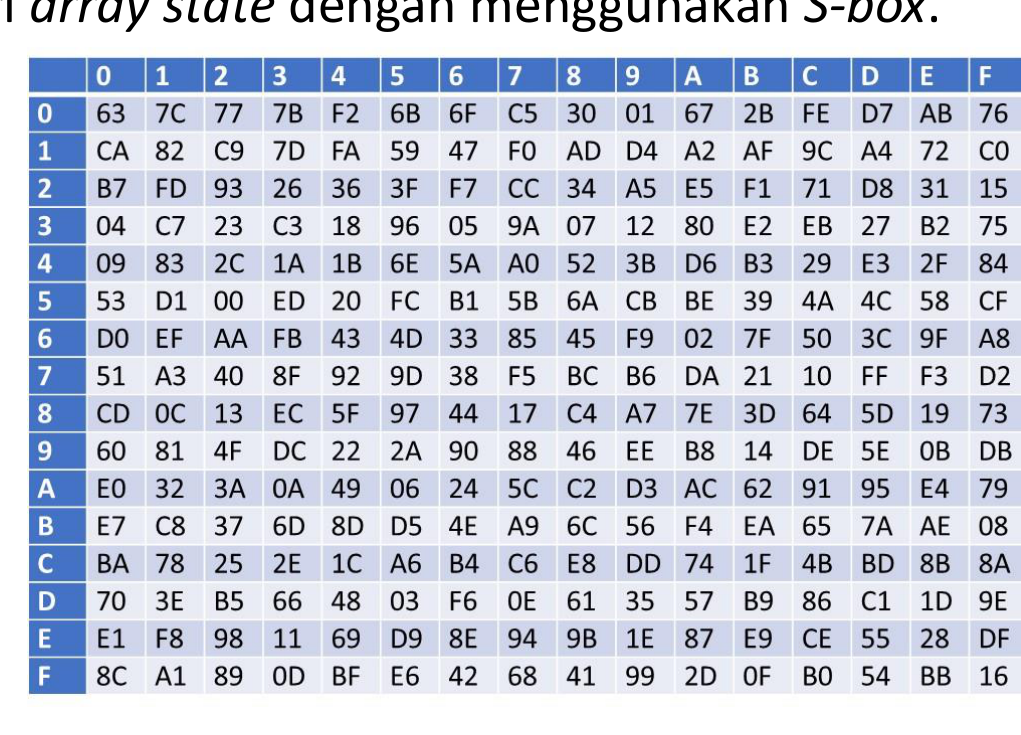
\includegraphics[width=111.72mm,height=202.26mm]{images/llm/page_018_img_01.png}%
\end{textblock*}

\newpage

% --- unit llm 19 ---
% === Halaman 19 (llm) ===

\vspace{151.47mm}

\vspace{50mm}
\begin{center}
Transformasi $SubBytes$
\end{center}

% deskripsi: Diagram proses transformasi SubBytes pada AES yang menunjukkan pemetaan dari sebuah matriks 'state' (elemen a_ij) melalui sebuah S-box menjadi matriks 'state'' (elemen b_ij).
% bbox normalisasi: [0.1400, 0.1500, 0.8400, 0.6600]
\begin{textblock*}{147.00mm}(29.40mm,44.55mm)
\noindent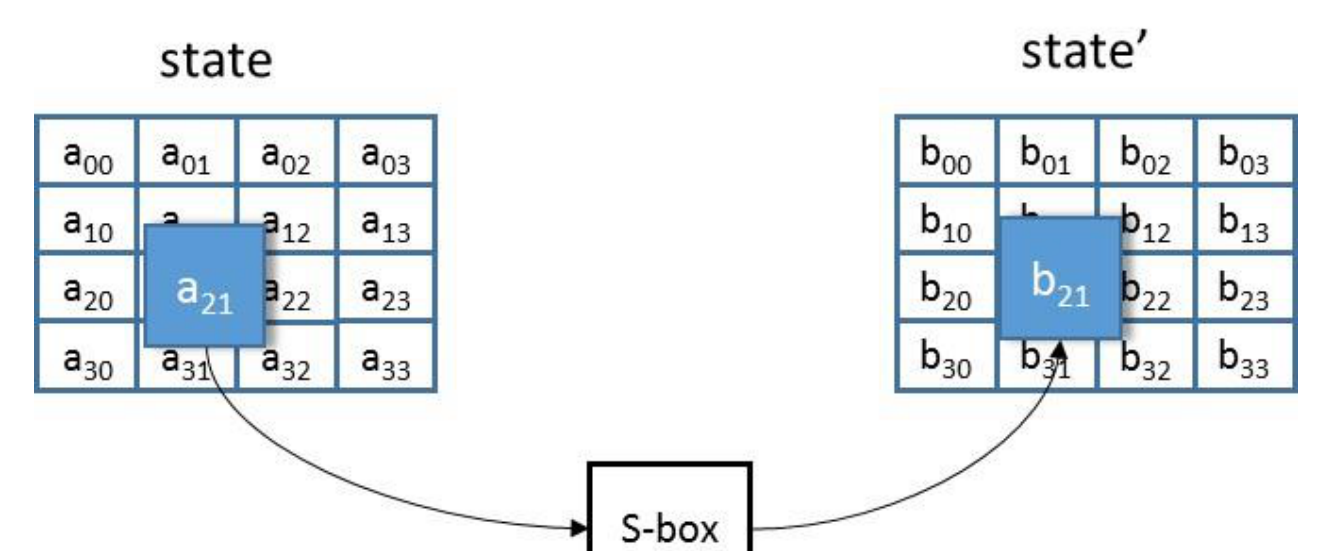
\includegraphics[width=147.00mm,height=151.47mm]{images/llm/page_019_img_01.png}%
\end{textblock*}

\newpage

% --- unit llm 20 ---
% === Halaman 20 (llm) ===

\vspace{163.35mm}

Contoh:\vspace{50mm}
Proses substitusi 23 menjadi 26

% deskripsi: Ilustrasi transisi antara dua state berupa matriks 4x4 dengan panah di antaranya, menunjukkan perubahan nilai tertentu.
% bbox normalisasi: [0.1900, 0.2100, 0.6500, 0.3100]
\begin{textblock*}{96.60mm}(39.90mm,62.37mm)
\noindent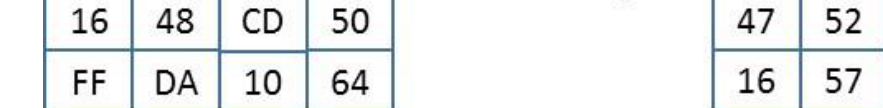
\includegraphics[width=96.60mm,height=29.70mm]{images/llm/page_020_img_01.png}%
\end{textblock*}

% deskripsi: Tabel substitusi S-Box yang berisi pemetaan nilai heksadesimal dari baris 0-F dan kolom 0-F.
% bbox normalisasi: [0.1800, 0.3700, 0.7900, 0.9200]
\begin{textblock*}{128.10mm}(37.80mm,109.89mm)
\noindent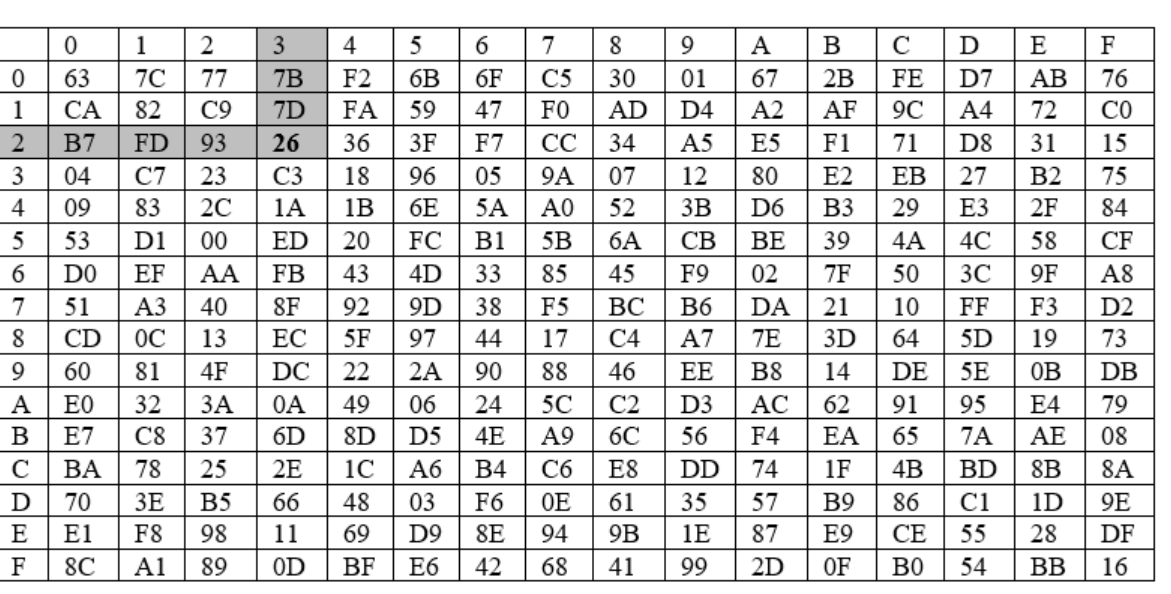
\includegraphics[width=128.10mm,height=163.35mm]{images/llm/page_020_img_02.png}%
\end{textblock*}

\newpage

% --- unit llm 21 ---
% === Halaman 21 (llm) ===

\section*{Transformasi $ShiftRows()$}

\vspace{158.00mm}

\begin{itemize}
    \item Transformasi $ShiftRows()$ melakukan operasi permutasi dengan pergeseran secara $wrapping$ (siklik) pada 3 baris terakhir array state.
    \item Jumlah pergeseran bergantung pada nilai baris ($r$). Baris $r = 1$ digeser sejauh 1 $byte$, baris $r = 2$ sejauh 2 $byte$, dan baris $r = 3$ sejauh 3 $byte$. Baris $r = 0$ tidak digeser.
\end{itemize}

\vspace{10mm}

% deskripsi: Diagram ilustrasi transformasi ShiftRows pada array state, menunjukkan pergeseran siklik baris 1, 2, dan 3 dari matriks state ke state'.
% bbox normalisasi: [0.1080, 0.4140, 0.8880, 0.9460]
\begin{textblock*}{163.80mm}(22.68mm,122.96mm)
\noindent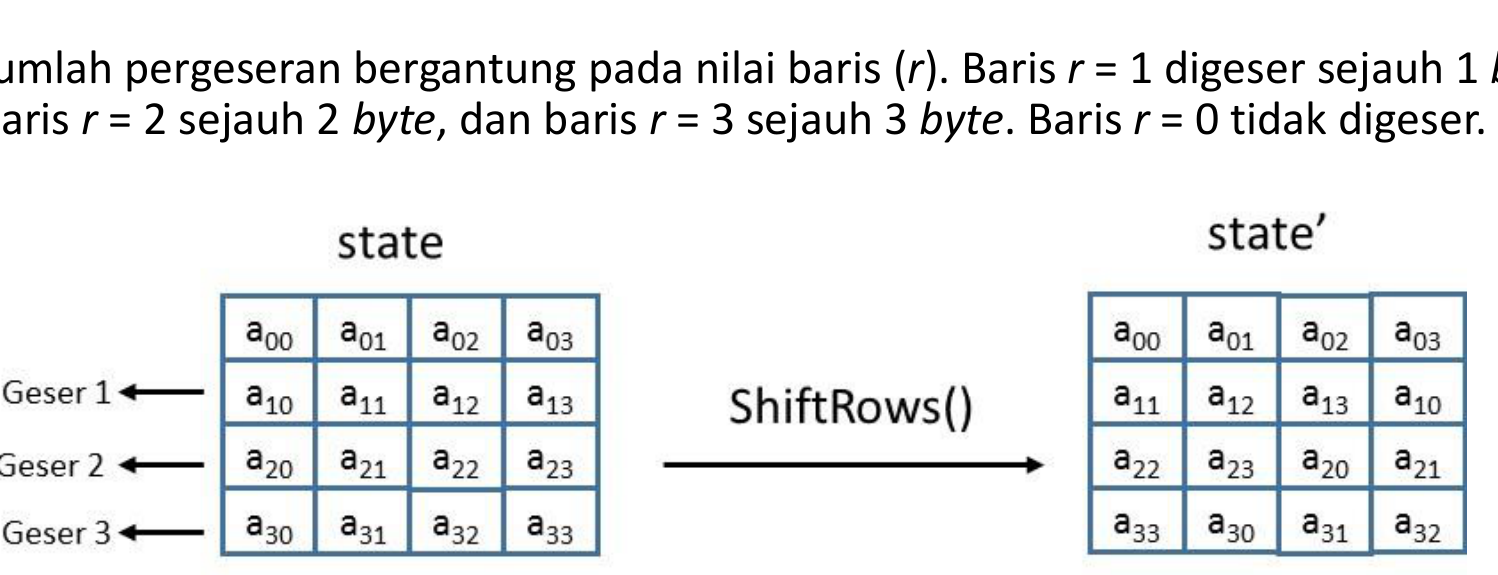
\includegraphics[width=163.80mm,height=158.00mm]{images/llm/page_021_img_01.png}%
\end{textblock*}

\newpage

% --- unit llm 22 ---
% === Halaman 22 (llm) ===

\vspace{83.16mm}

ShiftRows()

% deskripsi: Ilustrasi operasi ShiftRows pada matriks state dalam algoritma AES, menunjukkan pergeseran baris secara siklik ke kiri.
% bbox normalisasi: [0.1600, 0.2700, 0.8200, 0.5500]
\begin{textblock*}{138.60mm}(33.60mm,80.19mm)
\noindent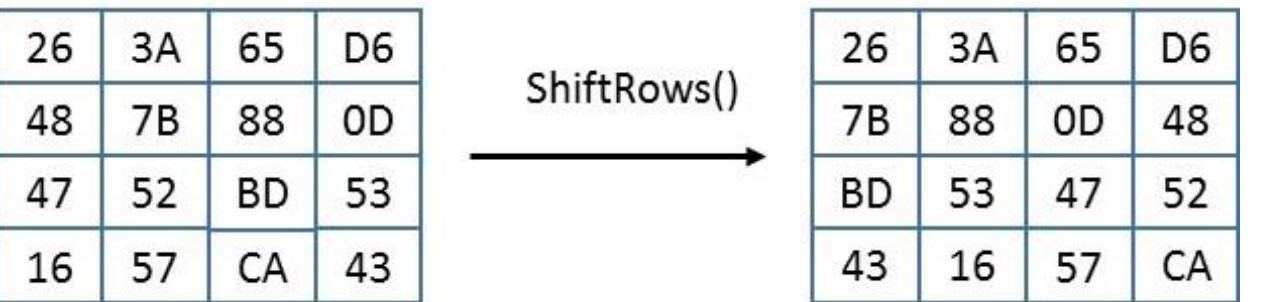
\includegraphics[width=138.60mm,height=83.16mm]{images/llm/page_022_img_01.png}%
\end{textblock*}

\newpage

% --- unit llm 23 ---
% === Halaman 23 (llm) ===

\vspace{238.79mm}

\section*{Transformasi $MixColumns()$}

\begin{itemize}
    \item Transformasi $MixColumns()$ mengalikan matriks $state$ dengan sebuah matriks tertentu sbb:
\end{itemize}

\vspace{5mm}

\[
\begin{bmatrix}
02 & 03 & 01 & 01 \\
01 & 02 & 03 & 01 \\
01 & 01 & 02 & 03 \\
03 & 01 & 01 & 02
\end{bmatrix} 
\begin{bmatrix}
s_{0,0} & s_{0,1} & s_{0,2} & s_{0,3} \\
s_{1,0} & s_{1,1} & s_{1,2} & s_{1,3} \\
s_{2,0} & s_{2,1} & s_{2,2} & s_{2,3} \\
s_{3,0} & s_{3,1} & s_{3,2} & s_{3,3}
\end{bmatrix} = 
\begin{bmatrix}
s'_{0,0} & s'_{0,1} & s'_{0,2} & s'_{0,3} \\
s'_{1,0} & s'_{1,1} & s'_{1,2} & s'_{1,3} \\
s'_{2,0} & s'_{2,1} & s'_{2,2} & s'_{2,3} \\
s'_{3,0} & s'_{3,1} & s'_{3,2} & s'_{3,3}
\end{bmatrix}
\]

% deskripsi: Persamaan perkalian matriks untuk transformasi MixColumns pada algoritma AES
% bbox normalisasi: [0.0600, 0.1080, 0.9400, 0.9120]
\begin{textblock*}{184.80mm}(12.60mm,32.08mm)
\noindent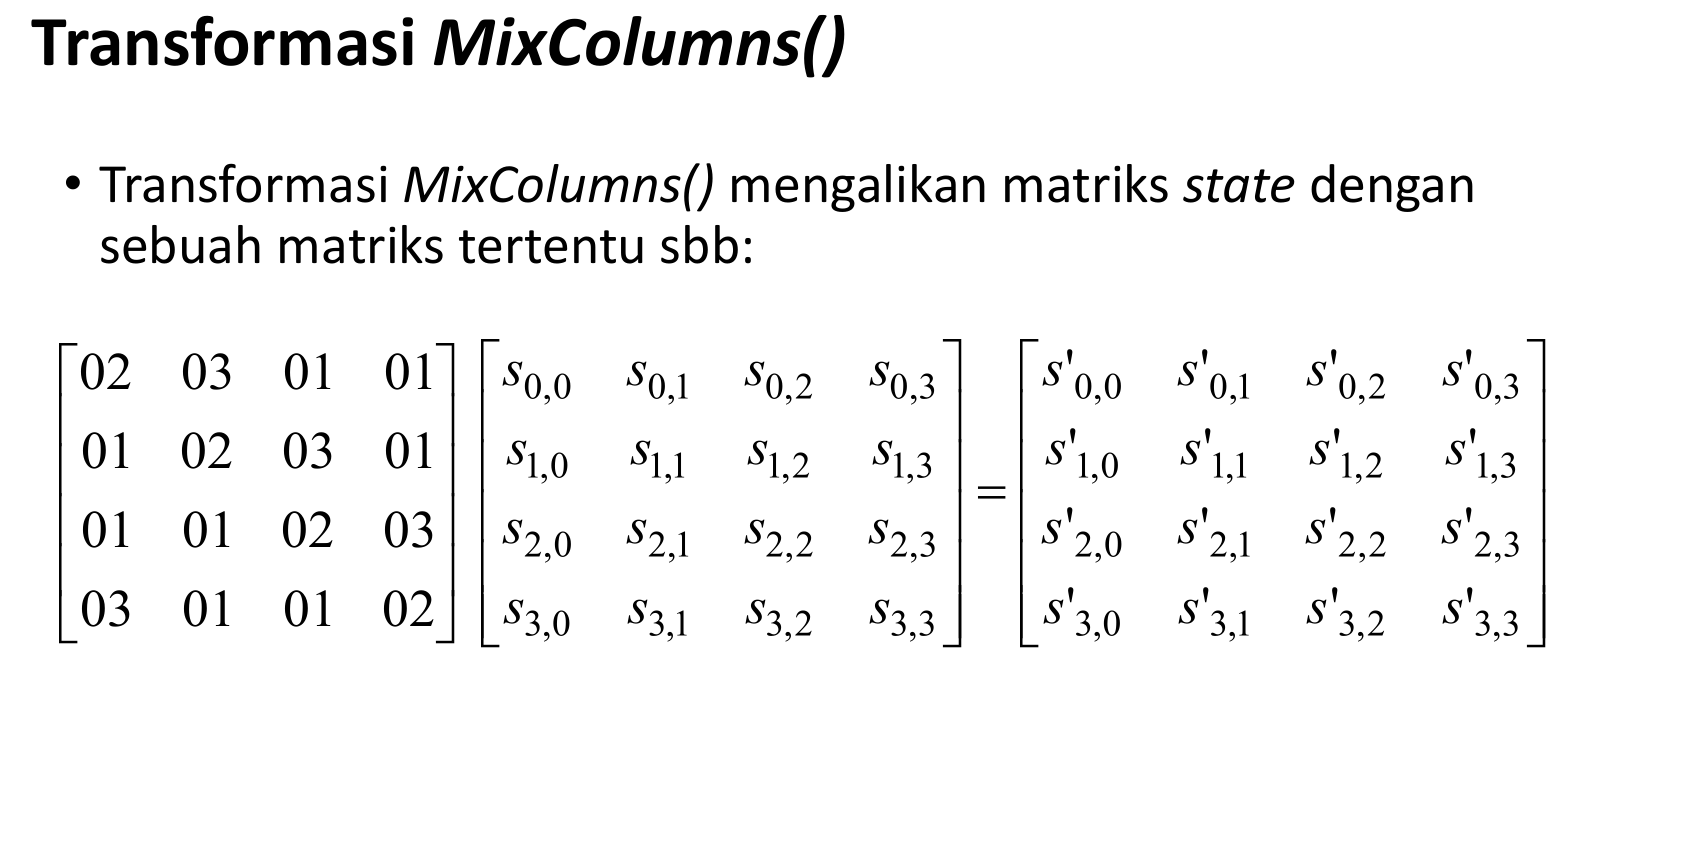
\includegraphics[width=184.80mm,height=238.79mm]{images/llm/page_023_img_01.png}%
\end{textblock*}

% bbox perkiraan otomatis: Persamaan perkalian matriks untuk transformasi MixColumns pada algoritma AES

\newpage

% --- unit llm 24 ---
% === Halaman 24 (llm) ===

\vspace{193.05mm}

state
\vspace{50mm}
\[
\begin{bmatrix}
02 & 03 & 01 & 01 \\
01 & 02 & 03 & 01 \\
01 & 01 & 02 & 03 \\
03 & 01 & 01 & 02
\end{bmatrix} = \begin{bmatrix} [ \ ] \\
[ \ ] \\
[ \ ] \\
[ \ ]
\end{bmatrix}
\]

% deskripsi: Diagram transisi state yang menunjukkan dua matriks elemen 'a' untuk 'state' dan elemen 'b' untuk 'state\'' dengan panah yang menghubungkan mereka ke sebuah matriks numerik di bagian bawah.
% bbox normalisasi: [0.1800, 0.2100, 0.8100, 0.8600]
\begin{textblock*}{132.30mm}(37.80mm,62.37mm)
\noindent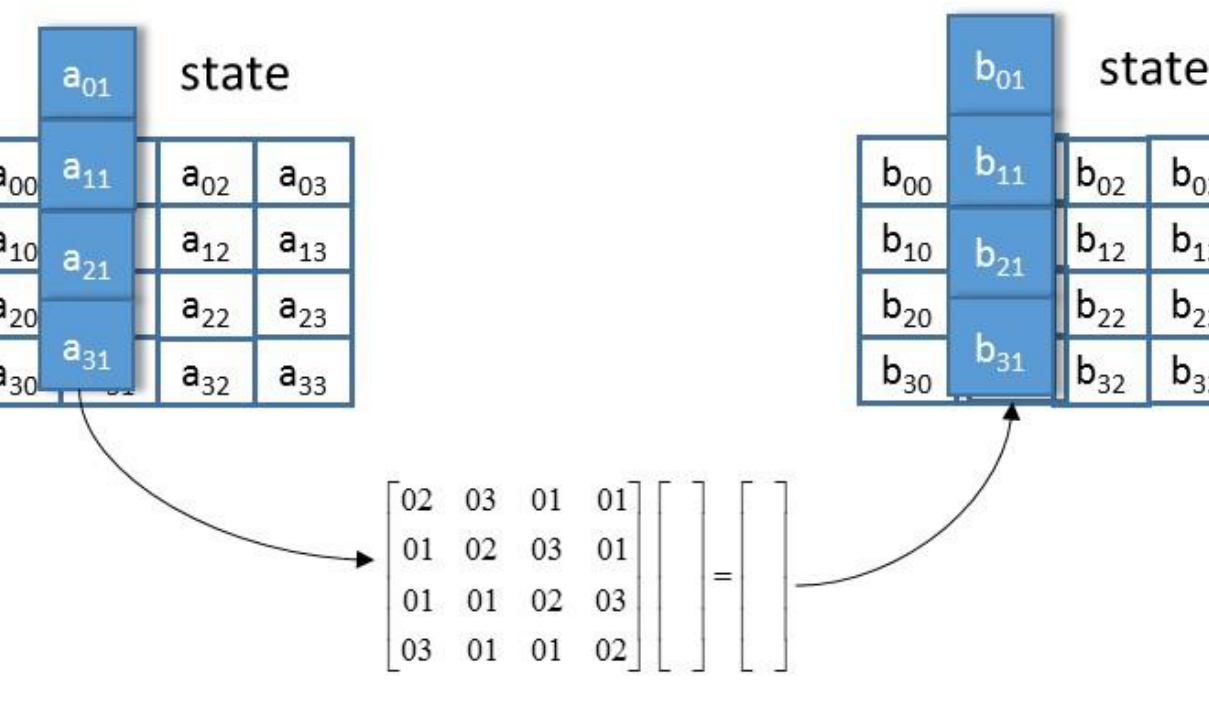
\includegraphics[width=132.30mm,height=193.05mm]{images/llm/page_024_img_01.png}%
\end{textblock*}

\newpage

% --- unit llm 25 ---
% === Halaman 25 (llm) ===

$s'(x) = a(x) \otimes s(x)$

\begin{equation*}
\begin{bmatrix}
s'_{0,c} \\ s'_{1,c} \\ s'_{2,c} \\ s'_{3,c}
\end{bmatrix} = \begin{bmatrix}
02 & 03 & 01 & 01 \\ 01 & 02 & 03 & 01 \\ 01 & 01 & 02 & 03 \\ 03 & 01 & 01 & 02
\end{bmatrix} \begin{bmatrix}
s_{0,c} \\ s_{1,c} \\ s_{2,c} \\ s_{3,c}
\end{bmatrix}
\end{equation*}

\begin{align*}
 s'_{0,c} &= (\{02\} \bullet s_{0,c}) \oplus (\{03\} \bullet s_{1,c}) \oplus s_{2,c} \oplus s_{3,c} \\
 s'_{1,c} &= s_{0,c} \oplus (\{02\} \bullet s_{1,c}) \oplus (\{03\} \bullet s_{2,c}) \oplus s_{3,c} \\
 s'_{2,c} &= s_{0,c} \oplus s_{1,c} \oplus (\{02\} \bullet s_{1,c}) \oplus (\{03\} \bullet s_{3,c}) \\
 s'_{3,c} &= (\{03\} \bullet s_{0,c}) \oplus s_{0,c} \oplus s_{1,c} \oplus (\{02\} \bullet s_{3,c}) 
\end{align*}

\newpage

% --- unit llm 26 ---
% === Halaman 26 (llm) ===

Contoh:

\vspace{10mm}

\vspace{10mm}

\begin{align*}
(02 \bullet 26) \oplus (03 \bullet 7\text{B}) \oplus (01 \bullet \text{BD}) \oplus (01 \bullet 43) &= 3\text{F} \\
(01 \bullet 26) \oplus (02 \bullet 7\text{B}) \oplus (03 \bullet \text{BD}) \oplus (01 \bullet 43) &= 4\text{F} \\
(01 \bullet 26) \oplus (01 \bullet 7\text{B}) \oplus (02 \bullet \text{BD}) \oplus (03 \bullet 43) &= \text{F}9 \\
(03 \bullet 26) \oplus (01 \bullet 7\text{B}) \oplus (01 \bullet \text{BD}) \oplus (02 \bullet 43) &= 2\text{A}
\end{align*}

Semua perkalian dan penjumlahan dilakukan dalam $\text{GF}(2^8)$

Penjelasan tentang $\text{GF}(2^m)$ dapat dilihat pada lampiran

% deskripsi: Operasi perkalian matriks dalam field GF(2^8) yang menunjukkan perkalian matriks 4x4 dengan vektor kolom 4x1 menghasilkan vektor kolom 4x1.
% bbox normalisasi: [0.1700, 0.1200, 0.5400, 0.4100]
\begin{textblock*}{77.70mm}(35.70mm,35.64mm)
\noindent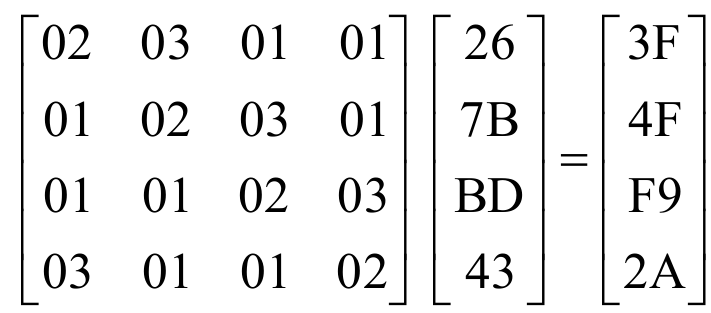
\includegraphics[width=77.70mm,height=86.13mm]{images/llm/page_026_img_01.png}%
\end{textblock*}

\newpage

% --- unit llm 27 ---
% === Halaman 27 (llm) ===

{\color{red} (02 \bullet 26) \oplus (03 \bullet 7B) \oplus (01 \bullet BD) \oplus (01 \bullet 43) = 3F}

\begin{align*}
(02 \bullet 26) &= (0000 \ 0010) \times (0010 \ 0110) \\
&= x \times (x^5 + x^2 + x) \pmod{x^8 + x^4 + x^3 + x + 1} \\
&= (x^6 + x^3 + x^2) \pmod{x^8 + x^4 + x^3 + x + 1} \\
&= x^6 + x^3 + x^2 \\
&= (01001100) \\
&= 4C
\end{align*}

\begin{align*}
(03 \bullet 7B) &= (0000 \ 0011) \times (0111 \ 1011) \\
&= (x + 1) \times (x^6 + x^5 + x^4 + x^3 + x + 1) \pmod{x^8 + x^4 + x^3 + x + 1} \\
&= ((x^7 + x^6 + x^5 + x^4 + x^2 + x) + (x^6 + x^5 + x^4 + x^3 + x + 1)) \pmod{x^8 + x^4 + x^3 + x + 1} \\
&= (x^7 + (1 + 1)x^6 + (1 + 1)x^5 + (1 + 1)x^4 + x^3 + x^2 + (1 + 1)x + 1) \pmod{x^8 + x^4 + x^3 + x + 1} \\
&= (x^7 + x^3 + x^2 + 1) \pmod{x^8 + x^4 + x^3 + x + 1} \\
&= (x^7 + x^3 + x^2 + 1) \\
&= (1000 \ 1101) = 8D
\end{align*}

\begin{align*}
(01 \bullet BD) &= BD = 10111101 \\
(01 \bullet 43) &= 43 = 01000011
\end{align*}

\newpage

% --- unit llm 28 ---
% === Halaman 28 (llm) ===

\textcolor{red}{(02 \bullet 26) \oplus (03 \bullet 7B) \oplus (01 \bullet BD) \oplus (01 \bullet 43) = 3F}

Selanjutnya, XOR-kan semua hasil antara tersebut:

\begin{align*}
(02 \bullet 26) &= 4C = 0100 \ 1100 \\
(03 \bullet 7B) &= 8D = 1000 \ 1101 \\
(01 \bullet BD) &= BD = 1011 \ 1101 \\
(01 \bullet 43) &= 43 = \underline{0100 \ 0011} \oplus \\
& \quad 0011 \ 1111 = 3F
\end{align*}

Jadi, $(02 \bullet 26) \oplus (03 \bullet 7B) \oplus (01 \bullet BD) \oplus (01 \bullet 43) = 3F$
Persamaan lainnya diselesaikan dengan cara yang sama.

\newpage

% --- unit llm 29 ---
% === Halaman 29 (llm) ===

\section*{Transformasi $AddRoundKey()$}

\vspace{95.04mm}

\begin{itemize}
    \item Transformasi ini melakukan operasi XOR antara \textit{round key} dan \textit{state}, dan hasilnya disimpan di \textit{state}.
\end{itemize}

\vspace{10mm}

% deskripsi: Diagram operasi XOR antara matriks 'state' dan 'round key' yang menghasilkan matriks 'state''
% bbox normalisasi: [0.1200, 0.4500, 0.8600, 0.7700]
\begin{textblock*}{155.40mm}(25.20mm,133.65mm)
\noindent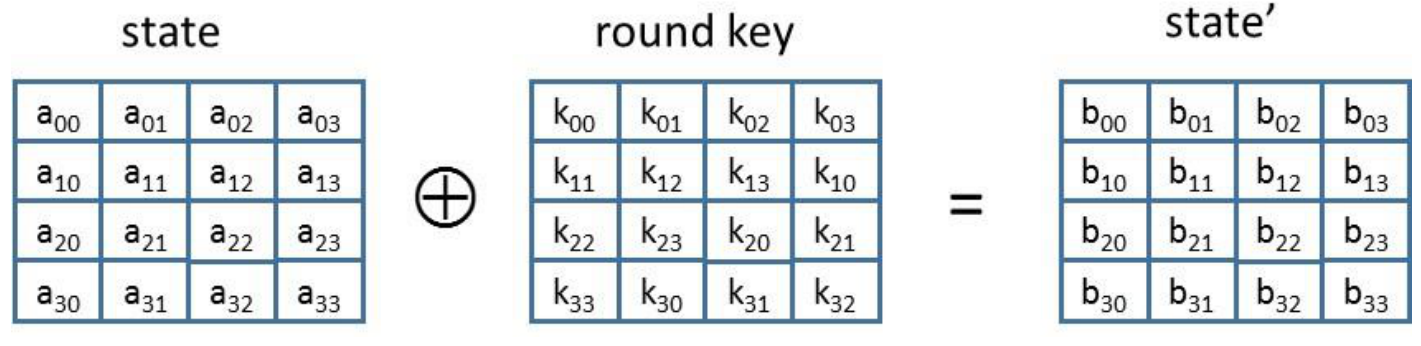
\includegraphics[width=155.40mm,height=95.04mm]{images/llm/page_029_img_01.png}%
\end{textblock*}

\newpage

% --- unit llm 30 ---
% === Halaman 30 (llm) ===

\vspace{87.91mm}

Contoh:\vspace{10mm}

% deskripsi: Operasi penjumlahan dua matriks berukuran 4x4 dengan elemen heksadesimal yang menghasilkan matriks hasil penjumlahan.
% bbox normalisasi: [0.1040, 0.3010, 0.9080, 0.5970]
\begin{textblock*}{168.84mm}(21.84mm,89.40mm)
\noindent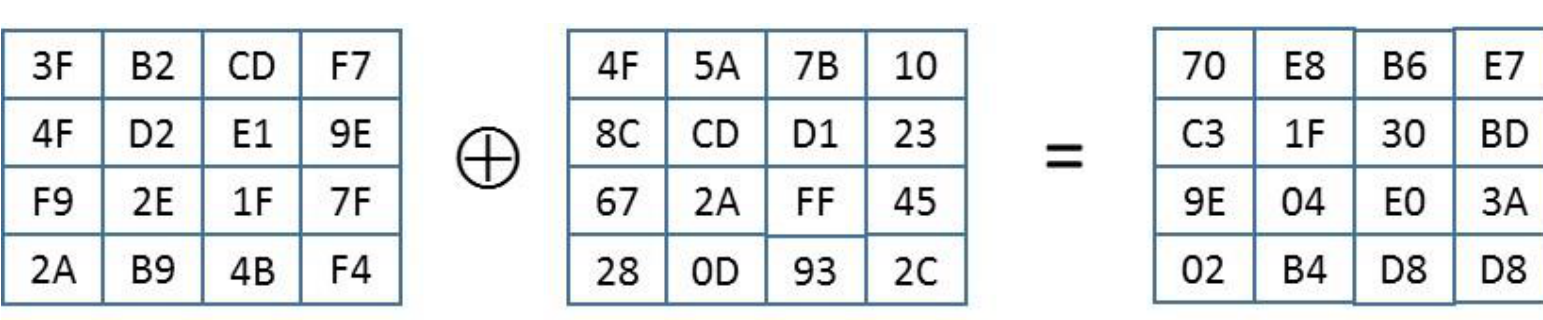
\includegraphics[width=168.84mm,height=87.91mm]{images/llm/page_030_img_01.png}%
\end{textblock*}

\newpage

% --- unit llm 31 ---
% === Halaman 31 (llm) ===

\section*{S-box}

Elemen-elemen di dalam $S\text{-}box$ terlihat seperti diisi secara acak, namun sebenarnya ia dihasilkan dari proses perhitungan sebagai berikut:

\begin{enumerate}
    \item Inisialisasi $S\text{-}box$ dengan nilai yang menaik dari baris ke baris. Baris ke-0 diisi dengan nilai 00, 01, 02, ..., 0F. Baris ke-1 diisi dengan nilai 10, 11, 12, ..., 1F, dan seterusnya untuk baris-baris lain.
    \item Untuk setiap nilai pada baris $y$ kolom $x$, tentukan balikannya dalam $\text{GF}(2^8)$. Nilai 00 dipetakan ke dirinya sendiri. Penjelasan tentang $\text{GF}(2^8)$ lihat pada lampiran.
    \item Hasil dari langkah 2 dikonversi ke vektor kolom bit $(b_0, b_1, ..., b_8)^\top$.
\end{enumerate}

\newpage

% --- unit llm 32 ---
% === Halaman 32 (llm) ===

4. Kalikan vektor kolom bit $(b_0, b_1, ..., b_8)^T$ dengan sebuah matriks \textit{affine} sebagai berikut:

\vspace{10mm}

5. Selanjutnya, konversi hasil perhitungan $(b'_0, b'_1, ..., b'_8)^T$ ke dalam heksadesimal, menjadi elemen $S\text{-}box(x, y)$.

% deskripsi: Persamaan perkalian matriks affine untuk transformasi bit dalam S-box, melibatkan matriks 8x8, vektor kolom b, dan vektor konstanta dengan operasi XOR.
% bbox normalisasi: [0.1860, 0.2660, 0.6840, 0.7340]
\begin{textblock*}{104.58mm}(39.06mm,79.00mm)
\noindent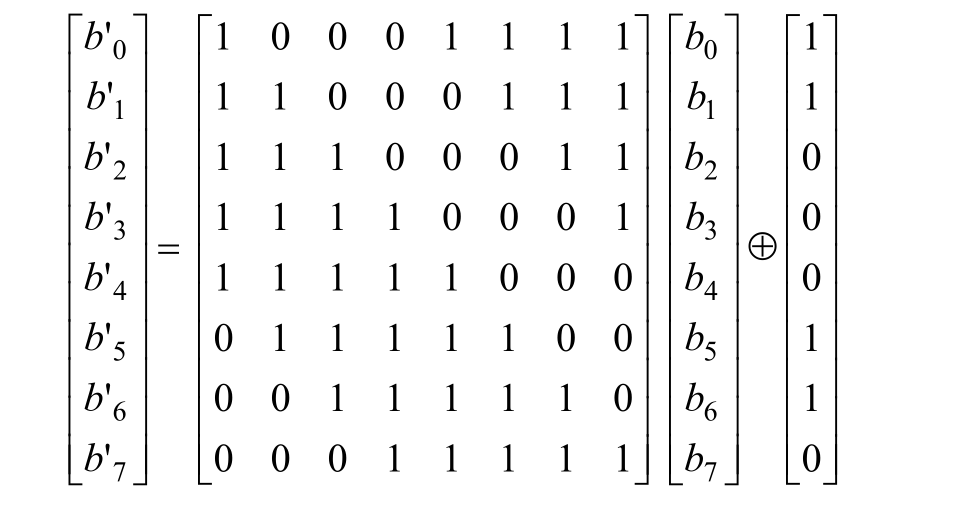
\includegraphics[width=104.58mm,height=139.00mm]{images/llm/page_032_img_01.png}%
\end{textblock*}

\newpage

% --- unit llm 33 ---
% === Halaman 33 (llm) ===

\vspace{70mm}

\begin{center}
{\Large S-box di dalam Rijndael}
\end{center}

% deskripsi: Tabel S-box yang digunakan dalam algoritma enkripsi Rijndael (AES), yang memetakan nilai input heksadesimal (baris dan kolom) ke nilai output heksadesimal.
% bbox normalisasi: [0.1300, 0.1100, 0.7600, 0.8300]
\begin{textblock*}{132.30mm}(27.30mm,32.67mm)
\noindent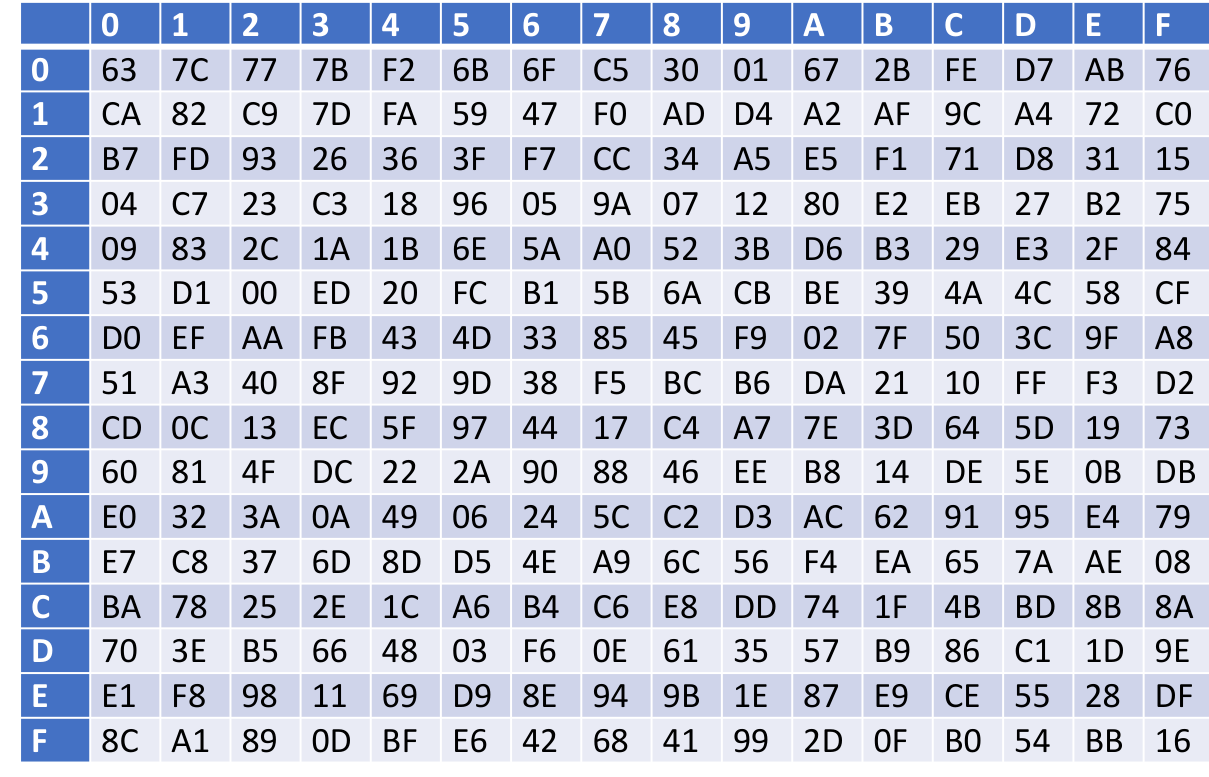
\includegraphics[width=132.30mm,height=213.84mm]{images/llm/page_033_img_01.png}%
\end{textblock*}

\newpage

% --- unit llm 34 ---
% === Halaman 34 (llm) ===

\section*{Pembentukan Kunci Putaran}

\begin{itemize}
    \item Setiap putaran di dalam algoritma \textit{Rijndael} menggunakan kunci putaran atau \textit{round key}. Kunci putaran dibangkitkan dari kunci eksternal dari pengguna yang dinamakan \textit{cipher key} dan disimbolkan dengan peubah \textit{key}. Pembangkitan semua kunci putaran dilakukan oleh fungsi \textit{KeyExpansion()}.
    \item Pembangkitan kunci putaran di dalam Algoritma Rijndael tergolong rumit dan agak sukar diterangkan. Tinjau sebuah larik \textit{key} yang panjangnya 16 \textit{byte} (16 elemen) dan $Nr = 10$ putaran. Sepuluh kunci putaran akan disimpan di dalam larik \textit{rk}. Elemen awal \textit{key} langsung menjadi $rk[0]$. Elemen-elemen kunci lainnya akan disimpan di dalam $rk[1], rk[2], \dots, rk[10]$.
\end{itemize}

\newpage

% --- unit llm 35 ---
% === Halaman 35 (llm) ===

\section*{ExpansionKey()}

Algoritma:

\begin{enumerate}
    \item Salin elemen-elemen $key$ ke dalam larik $w[0], w[1], w[2], w[3]$. Larik $w[0]$ berisi empat elemen pertama $key$, $w[1]$ berisi empat elemen berikutnya, dan seterusnya.
    \item Mulai dari $i = 4$ sampai $43$, lakukan:
    \begin{enumerate}
        \item Simpan $w[i-1]$ ke dalam peubah $temp$
        \item Jika $i$ kelipatan 4, lakukan fungsi $g$ berikut:
        \begin{itemize}
            \item \textbf{RotWord}: Geser $w[i-1]$ satu $byte$ ke kiri secara sirkuler
            \item \textbf{SubWord}: Lakukan substitusi dengan $S\text{-box}$ terhadap hasil pergeseran tersebut
        \end{itemize}
    \end{enumerate}
\end{enumerate}

\newpage

% --- unit llm 36 ---
% === Halaman 36 (llm) ===

\begin{itemize}
    \item \textbf{XOR Rcon}: XOR-kan hasilnya dengan \textit{round constant} (Rcon) ke $i/4$ (atau $Rcon[i/4]$).
    \begin{itemize}
        \item Nilai $Rcon$ berbeda-beda untuk setiap $j = i/4$, yaitu $Rcon[j] = (RC[j], 0, 0, 0)$, dengan $RC[1]=1, RC[j] = 2 \bullet RC[j-1]$, simbol $\bullet$ menyatakan perkalian yang didefinisikan di dalam $\text{GF}(2^8)$.
        \item Nilai $RC[j]$ di dalam heksadesimal adalah [STA11]: $RC[1]=01, RC[2]=02, RC[3]=04, RC[4]=08, RC[5]=10, RC[6]=20, RC[7]=40, RC[8]=80, RC[9]=1B, RC[10]=36$.
    \end{itemize}
    \item Simpan hasil fungsi $g$ ke dalam peubah \textit{temp}
\end{itemize}

\begin{enumerate}[label=\alph*)]
    \setcounter{enumi}{2}
    \item XOR-kan $w[i-4]$ dengan \textit{temp}
\end{enumerate}

\newpage

% --- unit llm 37 ---
% === Halaman 37 (llm) ===

Sebagai contoh, misalkan $key$ dalam hekadesimal adalah

\[ key = (54, 77, 6F, 20, 4F, 6E, 65, 20, 4E, 69, 6E, 65, 20, 54, 77, 6F) \]

\vspace{63.26mm}

Dari $key$ langsung diperoleh $rk[0]$ sebagai berikut:

\vspace{5mm}

% deskripsi: Tabel matriks yang berisi nilai heksadesimal hasil pemetaan dari kunci (key) menjadi rk[0].
% bbox normalisasi: [0.2820, 0.4520, 0.4910, 0.6650]
\begin{textblock*}{43.89mm}(59.22mm,134.24mm)
\noindent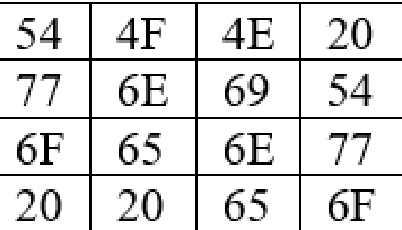
\includegraphics[width=43.89mm,height=63.26mm]{images/llm/page_037_img_01.png}%
\end{textblock*}

\newpage

% --- unit llm 38 ---
% === Halaman 38 (llm) ===

Proses di bawah ini hanya menunjukkan pembangkitan $rk[1]$:

\begin{enumerate}
    \item $w[0] = (54, 77, 6F, 20)$; $w[1] = (4F, 6E, 65, 20)$; $w[2] = (4E, 69, 6E, 65)$; \\
    $w[3] = (20, 54, 77, 6F)$
    \item Mulai dari $i = 4$:
    \begin{enumerate}
        \item $temp = w[3]$
        \item $i = 4$ adalah kelipatan 4, maka jalankan fungsi g terhadap $w[3]$:
        \begin{itemize}
            \item Geser $w[3]$ satu $byte$ ke kiri secara sirkuler: $w[3] = (54, 77, 6E, 20)$
            \item Substitusi hasil pergeseran tersebut dengan $S\text{-}box$: $(20, F5, 9F, B7)$
            \item XOR-kan hasil di atas dengan $Rcon[1] = (01, 00, 00, 00)$, menghasilkan $(21, F5, 9F, B7)$
        \end{itemize}
        Jadi, $g(w[3]) = (21, F5, 9F, B7)$
        \item $w[4] = w[0] \oplus g(w[3]) = w[0] \oplus g(w[3]) = (75, 82, F0, 97)$
    \end{enumerate}

    Untuk $i = 5, 6, 7$:
    \[
    \begin{aligned}
    w[5] &= w[4] \oplus w[1] = (3A, EC, 96, B7), \\
    w[6] &= w[5] \oplus w[2] = (74, 85, F8, D2), \\
    w[7] &= w[6] \oplus w[3] = (54, D1, 8F, BD)
    \end{aligned}
    \]
\end{enumerate}

Dari proses di atas diperoleh $rk[1]$ sebagai berikut:

\vspace{10mm}

% deskripsi: Tabel hasil pembangkitan round key rk[1] yang terdiri dari nilai-nilai hexadecimal dalam grid 4x4.
% bbox normalisasi: [0.3240, 0.7980, 0.5940, 0.9410]
\begin{textblock*}{56.70mm}(68.04mm,237.01mm)
\noindent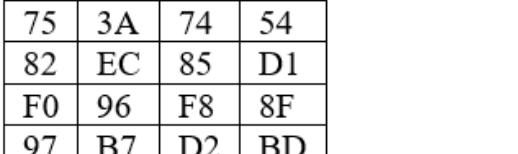
\includegraphics[width=56.70mm,height=42.47mm]{images/llm/page_038_img_01.png}%
\end{textblock*}

\newpage

% --- unit llm 39 ---
% === Halaman 39 (llm) ===

\vspace{160.38mm}

\section*{Dekripsi}

% deskripsi: Potongan kode program C++ untuk implementasi proses dekripsi algoritma Rijndael (AES), mencakup definisi konstanta, fungsi decrypt\_rijndael, dan langkah-langkah seperti InvShiftRows, InvSubBytes, AddRoundKey, dan InvMixColumns.
% bbox normalisasi: [0.2900, 0.4000, 0.9100, 0.9400]
\begin{textblock*}{130.20mm}(60.90mm,118.80mm)
\noindent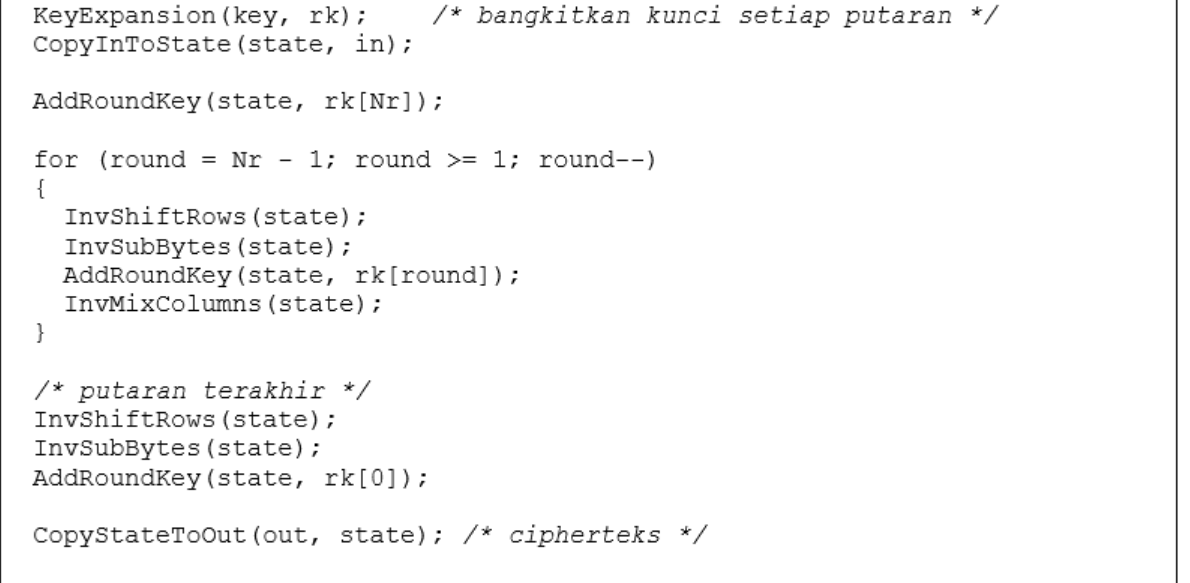
\includegraphics[width=130.20mm,height=160.38mm]{images/llm/page_039_img_01.png}%
\end{textblock*}

\newpage

% --- unit llm 40 ---
% === Halaman 40 (llm) ===

\section*{InvSubBytes()}

\vspace{160.38mm}

\begin{itemize}
    \item $InvSubBytes()$ sama seperti di dalam $SubBytes()$, hanya saja S-box yang digunakan adalah inversi dari S-box
\end{itemize}

\vspace{10mm}

\centerline{Gambar 6.27 Inversi S-box di dalam Rijndael}

% deskripsi: Tabel inversi S-box yang digunakan dalam algoritma enkripsi Rijndael/AES, menampilkan pemetaan nilai heksadesimal dari indeks baris dan kolom ke nilai hasil inversi.
% bbox normalisasi: [0.1500, 0.3300, 0.8300, 0.8700]
\begin{textblock*}{142.80mm}(31.50mm,98.01mm)
\noindent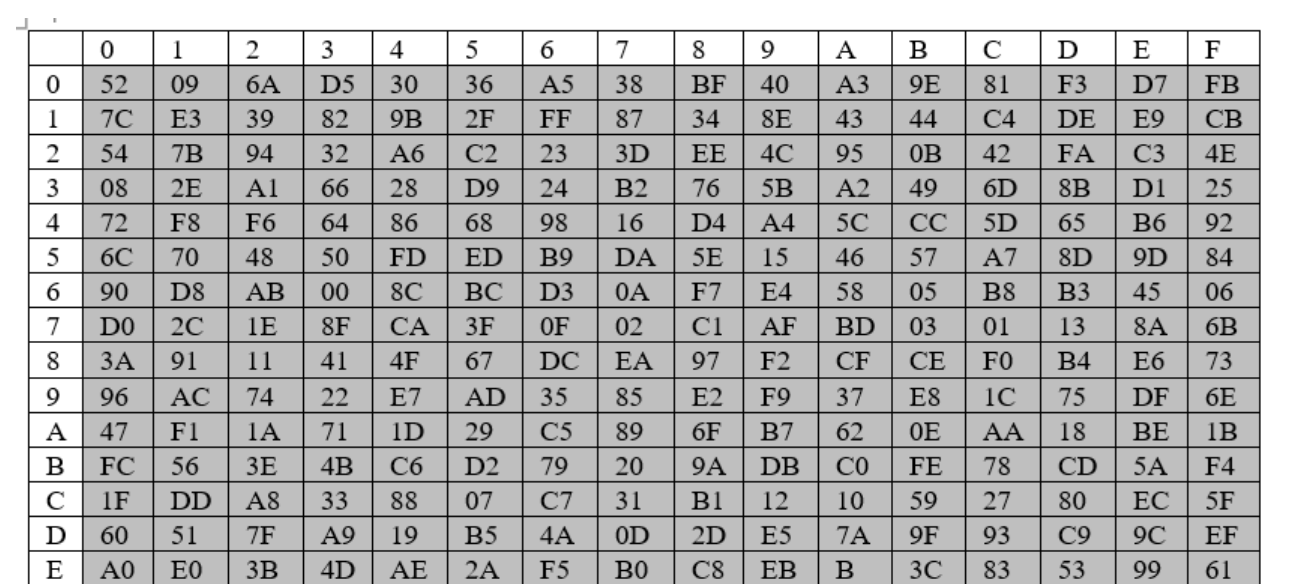
\includegraphics[width=142.80mm,height=160.38mm]{images/llm/page_040_img_01.png}%
\end{textblock*}

\newpage

% --- unit llm 41 ---
% === Halaman 41 (llm) ===

\section*{InvShiftRows()}

\begin{itemize}
    \item \textit{InvShiftRows} sama seperti \textit{ShiftRows} namun melakukan pergeseran dalam arah berlawanan (ke kanan) untuk tiap-tiap baris pada tiga baris terakhir di dalam \textit{state}
\end{itemize}

\vspace{10mm}

% deskripsi: Diagram ilustrasi proses InvShiftRows yang menunjukkan transformasi matriks state dari bentuk awal ke bentuk setelah pergeseran kanan pada baris kedua, ketiga, dan keempat.
% bbox normalisasi: [0.1300, 0.5000, 0.8500, 0.7500]
\begin{textblock*}{151.20mm}(27.30mm,148.50mm)
\noindent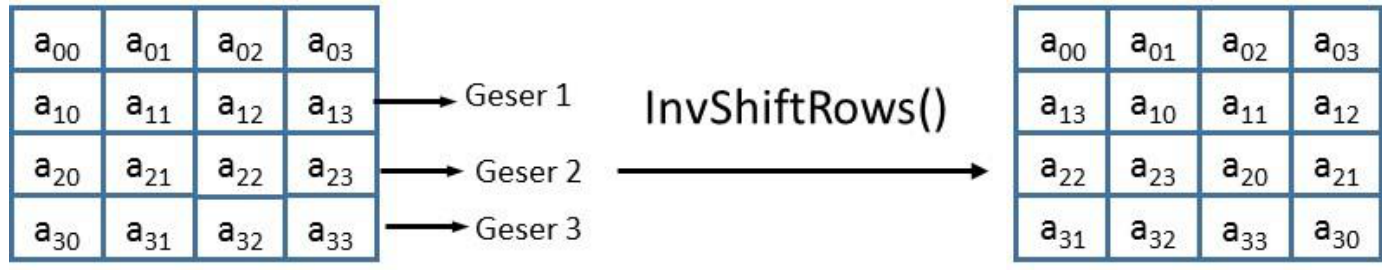
\includegraphics[width=151.20mm,height=74.25mm]{images/llm/page_041_img_01.png}%
\end{textblock*}

\newpage

% --- unit llm 42 ---
% === Halaman 42 (llm) ===

\section*{InvMixColumns()}

\vspace{10mm}

\[
\begin{bmatrix}
0\text{E} & 0\text{B} & 0\text{D} & 09 \\
09 & 0\text{E} & 0\text{B} & 0\text{D} \\
0\text{D} & 09 & 0\text{E} & 0\text{B} \\
0\text{B} & 0\text{D} & 09 & 0\text{E}
\end{bmatrix}
\begin{bmatrix}
s_{0,0} & s_{0,1} & s_{0,2} & s_{0,3} \\
s_{1,0} & s_{1,1} & s_{1,2} & s_{1,3} \\
s_{2,0} & s_{2,1} & s_{2,2} & s_{2,3} \\
s_{3,0} & s_{3,1} & s_{3,2} & s_{3,3}
\end{bmatrix} = 
\begin{bmatrix}
s'_{0,0} & s'_{0,1} & s'_{0,2} & s'_{0,3} \\
s'_{1,0} & s'_{1,1} & s'_{1,2} & s'_{1,3} \\
s'_{2,0} & s'_{2,1} & s'_{2,2} & s'_{2,3} \\
s'_{3,0} & s'_{3,1} & s'_{3,2} & s'_{3,3}
\end{bmatrix}
\]

% deskripsi: Persamaan matriks untuk operasi InvMixColumns dalam algoritma AES, menunjukkan perkalian matriks konstanta dengan matriks state s untuk menghasilkan state baru s'.
% bbox normalisasi: [0.1020, 0.3600, 0.8870, 0.6420]
\begin{textblock*}{164.85mm}(21.42mm,106.92mm)
\noindent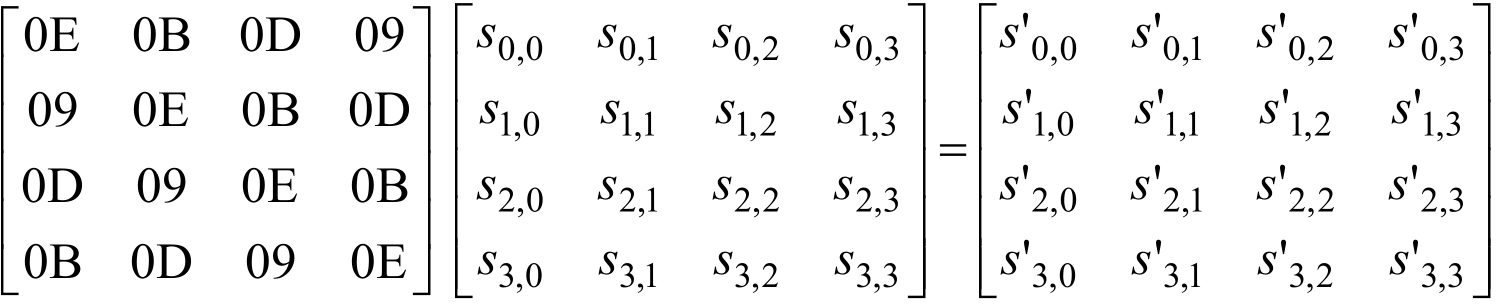
\includegraphics[width=164.85mm,height=83.75mm]{images/llm/page_042_img_01.png}%
\end{textblock*}

\newpage

% --- unit llm 43 ---
% === Halaman 43 (llm) ===

URL yang terkait dengan AES:
\begin{enumerate}
    \item AES Homepage, \url{http://www.nist.gov/CryptoToolkit}
    \item J. Daemen, V. Rijmen, AES Proposal: Rijndael, \url{http://www.esat.kuleuven.ac.be/~rizmen/}
\end{enumerate}

\newpage

% --- unit llm 44 ---
% === Halaman 44 (llm) ===

\section*{AES-256}

\begin{itemize}
    \item AES-256 dengan AES-128 hanya berbeda dalam hal:
    \begin{enumerate}
        \item Jumlah putaran 14 kali (AES-128 hanya 10 kali)
        \item Panjang kunci 256 bit (AES-128 hanya 128 bit)
        \item \textit{Expansion key} (untuk membangkitkan kunci putaran)
    \end{enumerate}

    \item \textit{Expansion key} pada AES-128 uritannya adalah sebagai berikut:
    
    RotWord $\rightarrow$ SubWord $\rightarrow$ XOR Rcon $\rightarrow$ XOR dengan word sebelumnya

    \item \textit{Expansion key} pada AES-256:
    
    Operasi SubWord tambahan pada word tertentu:
    
    jika $i \pmod 8 = 0$, dilakukan RotWord $\rightarrow$ SubWord $\rightarrow$ XOR Rcon
    
    jika $i \pmod 8 = 4$, dilakukan SubWord saja
\end{itemize}

\newpage

% --- unit llm 45 ---
% === Halaman 45 (llm) ===

\vspace{240.57mm}

Demo online AES \hfill \url{https://encode-decode.com/aes128-encrypt-online/}

\vspace{10mm}

% deskripsi: Screenshot halaman web alat enkripsi dan dekripsi AES-128 online dari situs encode-decode.com yang menunjukkan input teks berita dan hasil ciphertext.
% bbox normalisasi: [0.0600, 0.1400, 0.9300, 0.9500]
\begin{textblock*}{182.70mm}(12.60mm,41.58mm)
\noindent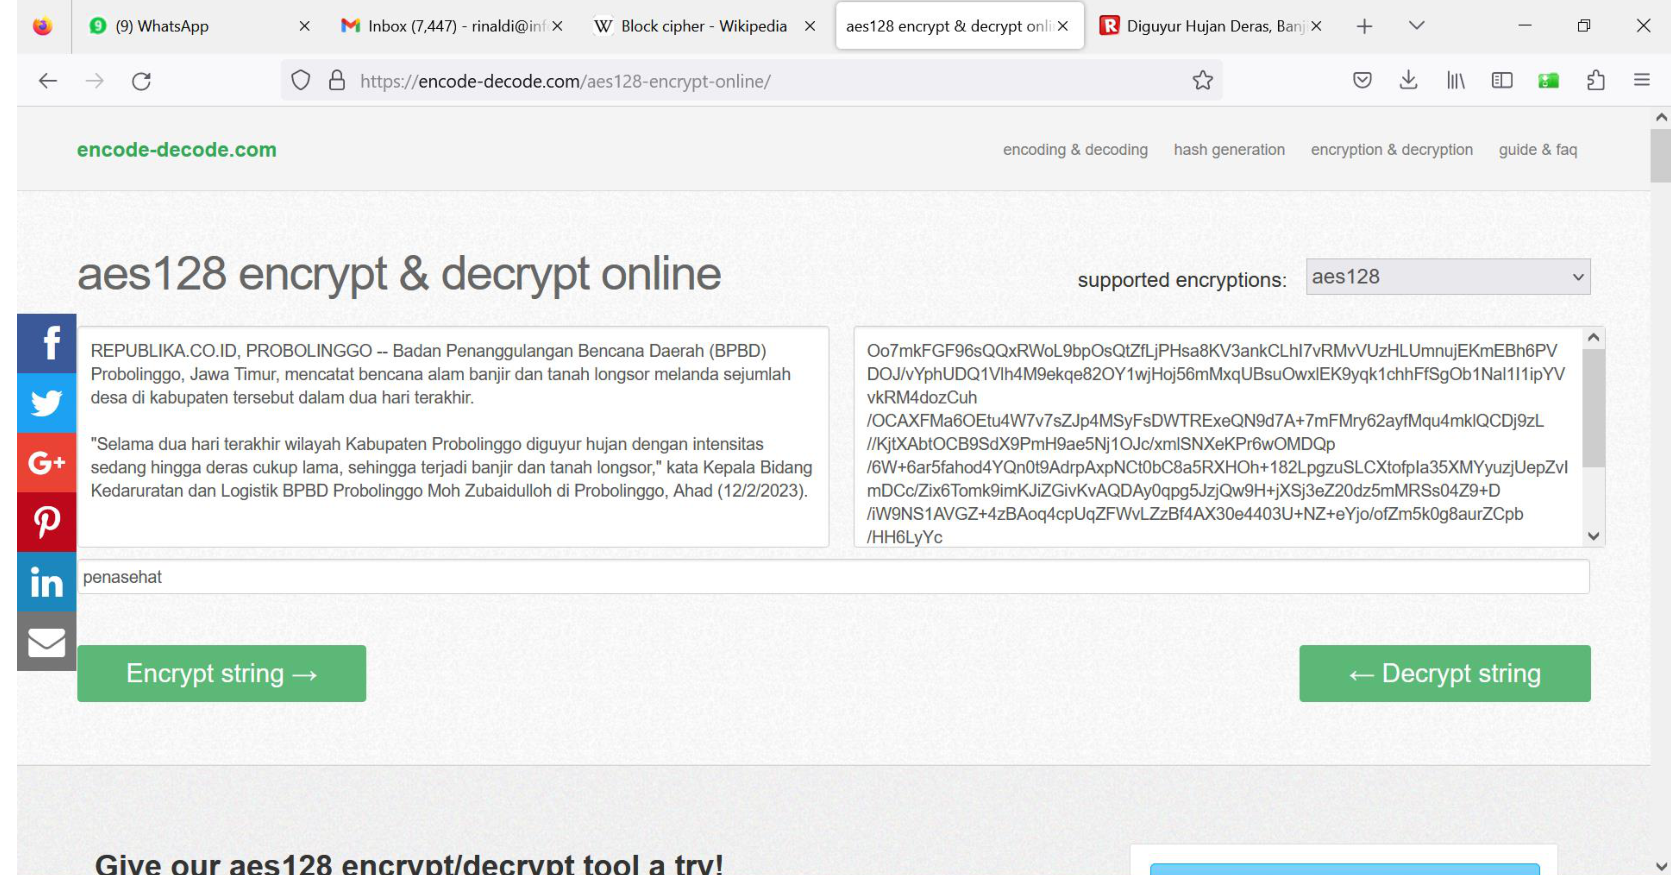
\includegraphics[width=182.70mm,height=240.57mm]{images/llm/page_045_img_01.png}%
\end{textblock*}

\newpage

% --- unit llm 46 ---
% === Halaman 46 (llm) ===

\section*{Program enkripsi-dekripsi AES dengan Python}
\textbf{Input: Teks dari keyboard}

\vspace{167.21mm}

\begin{verbatim}
from Crypto.Cipher import AES
from Crypto.Random import get_random_bytes
from Crypto.Util.Padding import pad, unpad
import base64

# Panjang blok AES
BLOCK_SIZE = 16

def enkripsi_aes(plainteks, kunci):
    kunci = kunci.encode()
    iv = get_random_bytes(BLOCK_SIZE)
    AEScipher = AES.new(kunci, AES.MODE_CBC, iv)

    plainteks = pad(plainteks.encode(), BLOCK_SIZE)

    cipherteks = AEScipher.encrypt(plainteks)
    cipherteks = base64.b64encode(iv+cipherteks)
    return cipherteks
\end{verbatim}

% deskripsi: Screenshot cuplikan kode Python untuk fungsi enkripsi AES menggunakan library PyCryptodome
% bbox normalisasi: [0.0480, 0.2310, 0.8900, 0.7940]
\begin{textblock*}{176.82mm}(10.08mm,68.61mm)
\noindent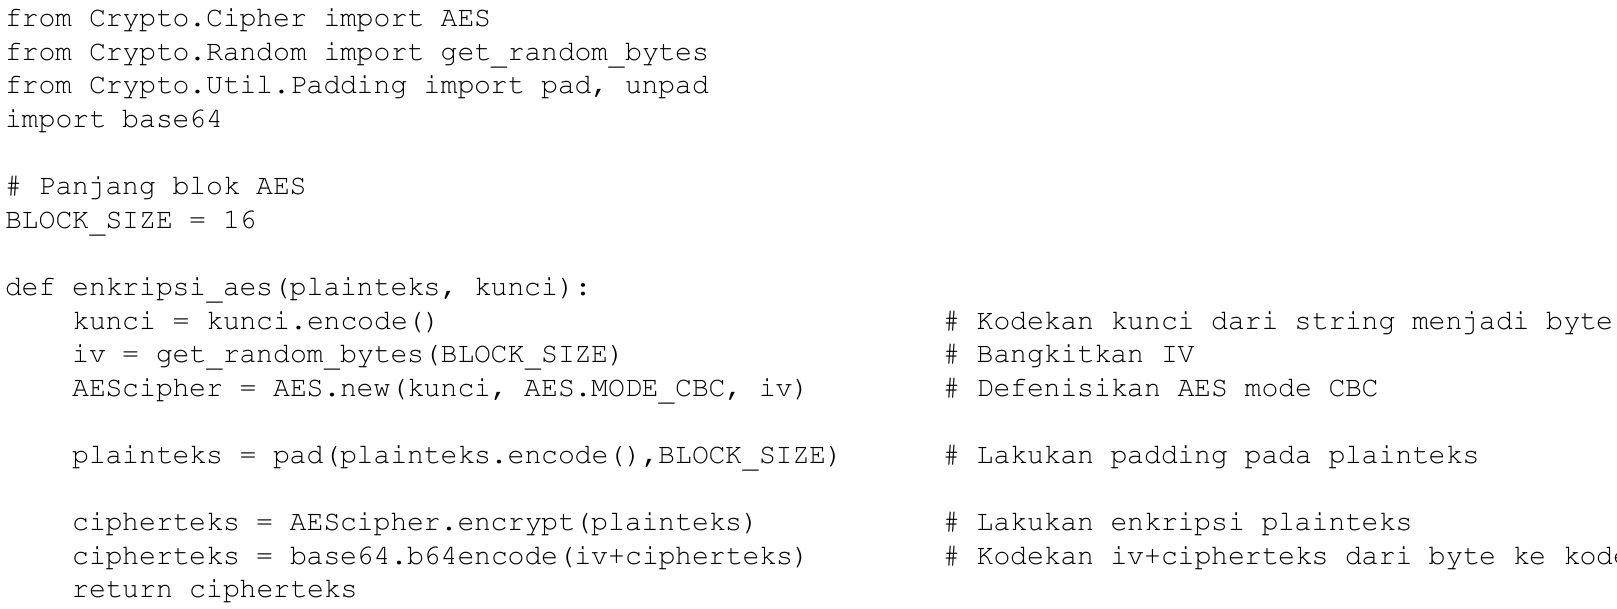
\includegraphics[width=176.82mm,height=167.21mm]{images/llm/page_046_img_01.png}%
\end{textblock*}

\newpage

% --- unit llm 47 ---
% === Halaman 47 (llm) ===

\vspace{228.69mm}

\begin{verbatim}
def dekripsi_aes(cipherteks, kunci):
    kunci = kunci.encode()
    cipherteks = base64.b64decode(cipherteks)
    iv = cipherteks[:16]
    AEScipher = AES.new(kunci, AES.MODE_CBC, iv)
    plainteks = AEScipher.decrypt(cipherteks[BLOCK_SIZE:])
    plainteks = unpad(plainteks, BLOCK_SIZE)
    return plainteks

# Program utama (pemanggilan fungsi enkripsi dan dekripsi AES)
# Enkripsi pesan
print("E N K R I P S I:")
pesan = input("Ketikkan pesan yang akan dienkripsi:")
kunci = input("Ketikkan kunci (harus sepanjang 16 karakter):")
cipherteks = enkripsi_aes(pesan, kunci)
print("Cipherteks hasil enkripsi: ", cipherteks)

# Dekripsi pesan
print("D E K R I P S I:")
kunci = input("Ketikkan kunci (harus sepanjang 16 karakter):")
plainteks = dekripsi_aes(cipherteks, kunci)
#plainteks = unpad(plainteks, BLOCK_SIZE)
print("Plainteks hasil dekripsi: ", plainteks[16:])
\end{verbatim}

% deskripsi: Screenshot potongan kode Python yang mengimplementasikan fungsi dekripsi AES dan alur program utama untuk enkripsi dan dekripsi.
% bbox normalisasi: [0.0700, 0.1400, 0.8900, 0.9100]
\begin{textblock*}{172.20mm}(14.70mm,41.58mm)
\noindent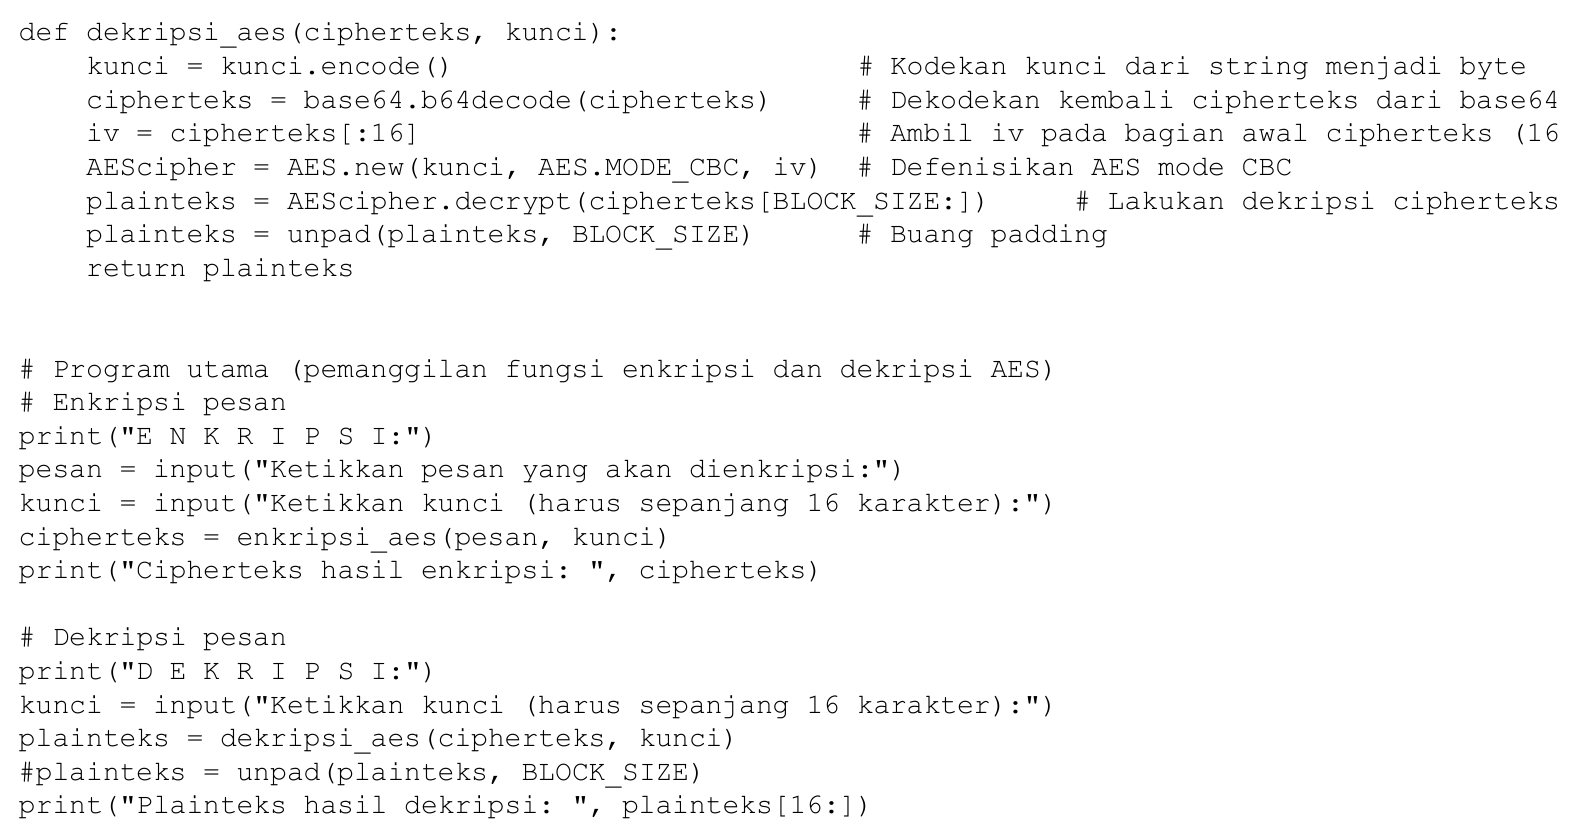
\includegraphics[width=172.20mm,height=228.69mm]{images/llm/page_047_img_01.png}%
\end{textblock*}

\newpage

% --- unit llm 48 ---
% === Halaman 48 (llm) ===

\section*{Running program}

ENKRIPSI:\
Ketikkan pesan yang akan dienkripsi: Besok tunggu saya di Stasiun Bandung pukul 17.30\
Ketikkan kunci (harus sepanjang 16 karakter): abcdefghij123456\
Cipherteks hasil enkripsi:\
b'WKOTLyCGVHb8sD0q15LCrQ PikUjSDjWupum05suL5cJvglZ6+XKoBNLCTVbLlm+DBSDE+yID/i5H16VSW1Km8P\nOeoqOSzi2EOGsDM2Ld7RY='\

DEKRIPSI:\
Ketikkan kunci (harus sepanjang 16 karakter): abcdefghij123456\
Plainteks hasil dekripsi: b'Besok tunggu saya di Stasiun Bandung pukul 17.30'

\newpage

% --- unit llm 49 ---
% === Halaman 49 (llm) ===

\section*{Program enkripsi-dekripsi AES dengan Python}
Input: File biner

\vspace{10mm}

\begin{verbatim}
# Enkripsi file biner dengan AES-128
from Crypto.Cipher import AES
from Crypto.Random import get_random_bytes
from Crypto.Util.Padding import pad, unpad
import base64

BLOCK_SIZE = 16           # Panjang blok pesan yang dienkripsi = 16 byte = 128 bit

def enkripsi_aes(plainteks, kunci):
    kunci = kunci.encode()                # Kodekan kunci dari string menjadi byte
    iv = get_random_bytes(BLOCK_SIZE)     # Bangkitkan IV
    AEScipher = AES.new(kunci, AES.MODE_CBC, iv) # Definisikan AES mode CBC

    plainteks = pad(plainteks, BLOCK_SIZE) # lakukan padding jika ukuran plainteks bukan kelipatan 16 byte

    cipherteks = AEScipher.encrypt(plainteks) # Lakukan enkripsi plainteks
    cipherteks = base64.b64encode(iv+cipherteks) # Kodekan iv+cipherteks dari kode byte ke base64
    return cipherteks
\end{verbatim}

\newpage

% --- unit llm 50 ---
% === Halaman 50 (llm) ===

\vspace{243.54mm}

def dekripsi\_aes(cipherteks, kunci):
    kunci = kunci.encode()
    cipherteks = base64.b64decode(cipherteks)
    iv = cipherteks[:16]
    AEScipher = AES.new(kunci, AES.MODE\_CBC, iv)
    plainteks = AEScipher.decrypt(cipherteks[BLOCK\_SIZE:])
    plainteks = unpad(plainteks, BLOCK\_SIZE)
    return plainteks

def encrypt\_file(input\_file, output\_file, key):
    with open(input\_file, 'rb') as f:
        plaintext = f.read()

    ciphertext = enkripsi\_aes(plaintext, key)

    with open(output\_file, 'wb') as f:
        f.write(ciphertext)

def decrypt\_file(input\_file, output\_file, key):
    with open(input\_file, 'rb') as f:
        ciphertext = f.read()

    plaintext = dekripsi\_aes(ciphertext, key)

    with open(output\_file, 'wb') as f:
        f.write(plaintext)

% deskripsi: Screenshot potongan kode Python untuk implementasi enkripsi dan dekripsi file menggunakan algoritma AES.
% bbox normalisasi: [0.0600, 0.0600, 0.8800, 0.8800]
\begin{textblock*}{172.20mm}(12.60mm,17.82mm)
\noindent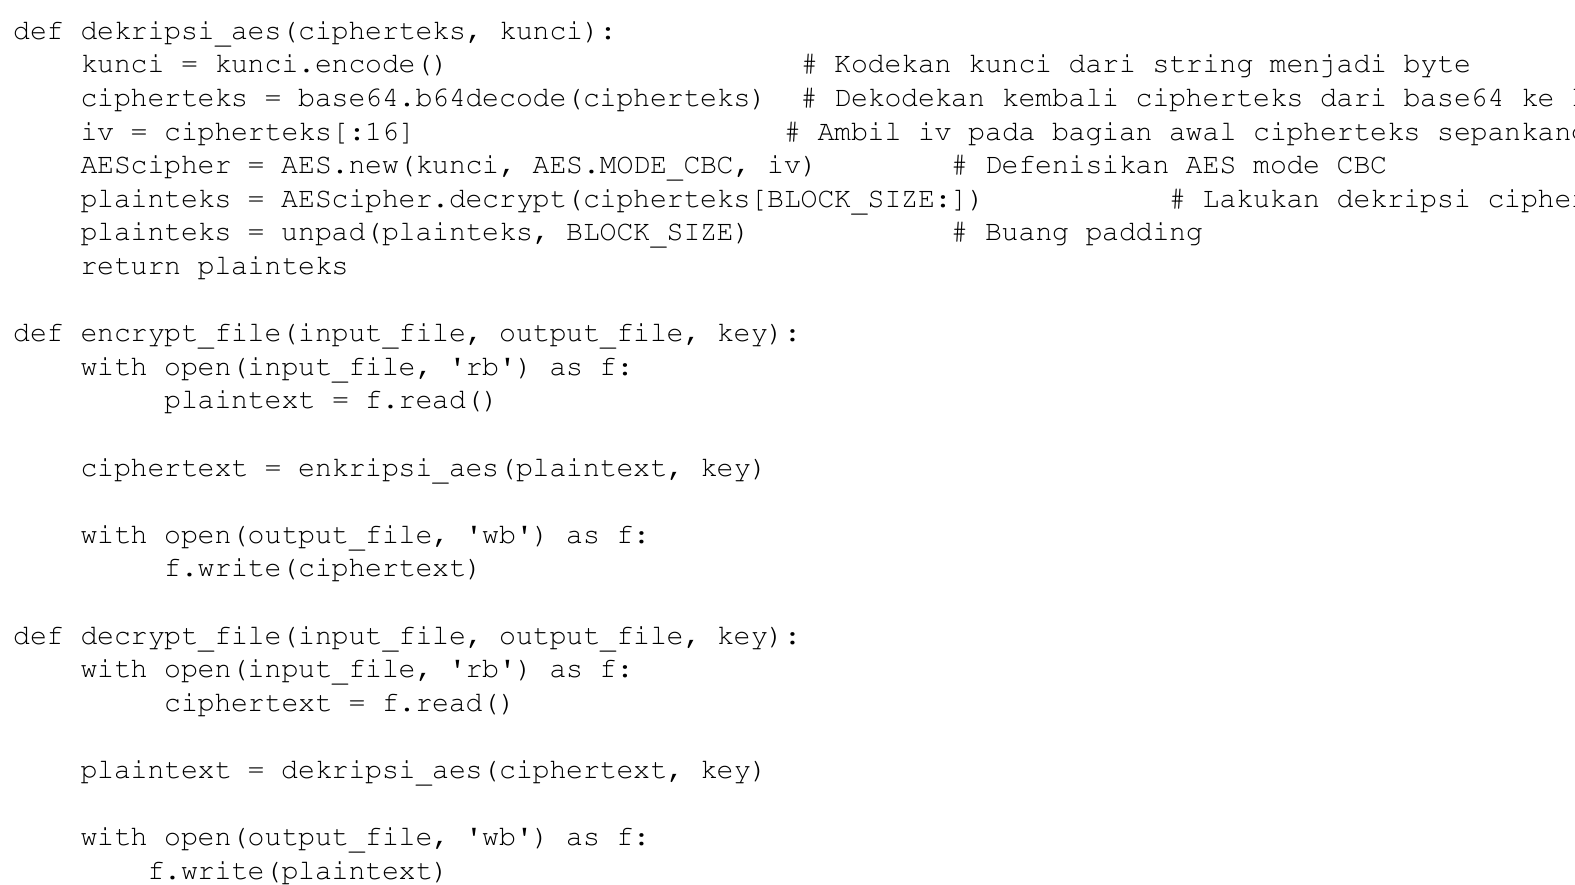
\includegraphics[width=172.20mm,height=243.54mm]{images/llm/page_050_img_01.png}%
\end{textblock*}

\newpage

% --- unit llm 51 ---
% === Halaman 51 (llm) ===

\vspace{103.95mm}

\begin{verbatim}
# Program utama (pemanggilan fungsi enkripsi dan dekripsi AES)
file_plaintext = input("Ketikkan nama file input pesan yang akan dienkripsi: (beserta path) ")
file_ciphertext = input("Ketikkan nama file output pesan hasil enkripsi (beserta path): ")
kunci = input("Kunci?:")
encrypt_file(file_plaintext, file_ciphertext, kunci)
print("Enkripsi selesai. Hasil disimpan di:", file_ciphertext)

file_ciphertext = input("Ketikkan nama file input pesan yang akan didekripsi: (beserta path) ")
file_plaintext = input("Ketikkan nama file output pesan hasil dekripsi (beserta path): ")
kunci = input("Kunci?:")
decrypt_file(file_ciphertext, file_plaintext, kunci)
print("Dekripsi selesai. Hasil disimpan di:", file_plaintext)
\end{verbatim}

% deskripsi: Potongan kode Python untuk implementasi program utama enkripsi dan dekripsi AES
% bbox normalisasi: [0.0400, 0.1900, 0.8800, 0.5400]
\begin{textblock*}{176.40mm}(8.40mm,56.43mm)
\noindent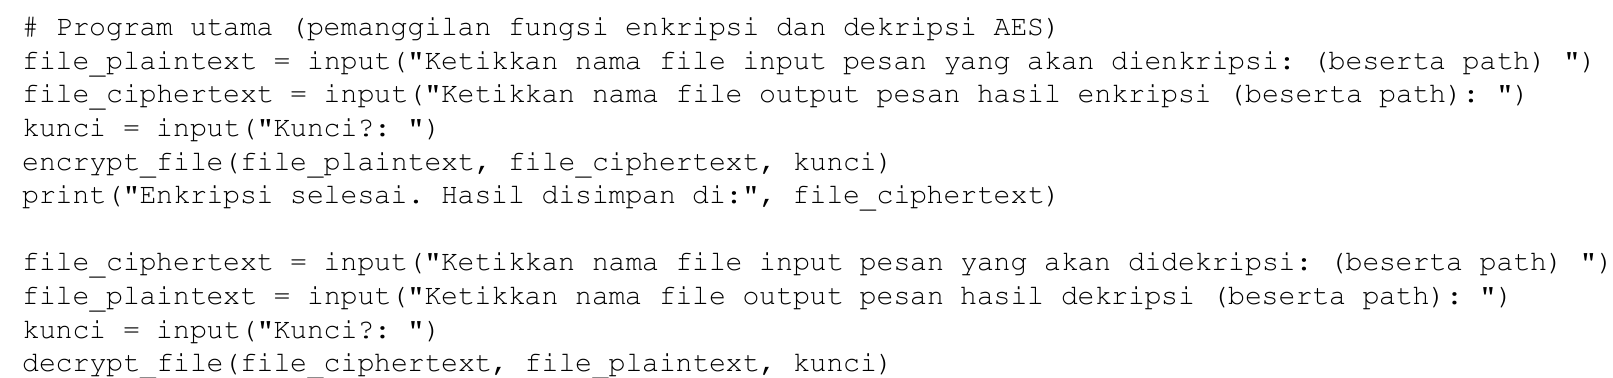
\includegraphics[width=176.40mm,height=103.95mm]{images/llm/page_051_img_01.png}%
\end{textblock*}

\newpage

% --- unit llm 52 ---
% === Halaman 52 (llm) ===

\section*{Running program}

Ketikkan nama file input pesan yang akan dienkripsi: (beserta path) E:\\STIN\\Kriptografi 2026\\01-Pengantar-Kriptografi-(2026).pdf\\
Ketikkan nama file output pesan hasil enkripsi (beserta path): E:\\STIN\\Kriptografi 2026\\01-Pengantar-Kriptografi-(2026).enc\\
Kunci?: abcdefghij123456

Enkripsi selesai. Hasil disimpan di: E:\\STIN\\Kriptografi 2026\\01-Pengantar-Kriptografi-(2026).enc

Ketikkan nama file input pesan yang akan didekripsi: (beserta path) E:\\STIN\\Kriptografi 2026\\01-Pengantar-Kriptografi-(2026).enc\\
Ketikkan nama file output pesan hasil dekripsi (beserta path): E:\\STIN\\Kriptografi 2026\\01-Pengantar-Kriptografi-(2026)-hasil.pdf\\
Kunci?: abcdefghij123456

Dekripsi selesai. Hasil disimpan di: E:\\STIN\\Kriptografi 2026\\01-Pengantar-Kriptografi-(2026)-hasil.pdf

\newpage

% --- unit llm 53 ---
% === Halaman 53 (llm) ===

Lampiran

\newpage

% --- unit llm 54 ---
% === Halaman 54 (llm) ===

\section*{Galois Field $\text{GF}(2^m)$}

\begin{itemize}
    \item Disebut juga medan berhingga biner.
    \item $\text{GF}(2^m)$ atau $\text{F}_{2^m}$ adalah ruang vektor berdimensi $m$ pada $\text{GF}(2)$. Setiap elemen di dalam $\text{GF}(2^m)$ adalah integer dalam representasi biner sepanjang maksimal $m$ bit.\
    Contoh: $\text{GF}(2^4)$, $\text{GF}(2^8)$, dst
    \item String biner $b_{m-1}b_{m-2} \dots b_1b_0$, $b_i \in \{0,1\}$, dapat dinyatakan sebagai polinom
    \[ b_{m-1}x^{m-1} + b_{m-2}x^{m-2} + \dots + b_1x + b_0 \]
    \item Jadi, setiap $a \in \text{GF}(2^m)$ dapat dinyatakan sebagai
    \[ b_{m-1}x^{m-1} + b_{m-2}x^{m-2} + \dots + b_1x + b_0 \]
    \item Contoh: 1101 di dalam $\text{GF}(2^4)$ dapat dinyatakan sebagai polinom $x^3 + x^2 + 1$\\
    01010111 di dalam $\text{GF}(2^8)$ dapat dinyatakan sebagai polinom $x^6 + x^4 + x^2 + x + 1$
\end{itemize}

\newpage

% --- unit llm 55 ---
% === Halaman 55 (llm) ===

\textbf{Operasi aritmetika pada $\text{GF}(2^m)$}

Misalkan $a = (a_{m-1} \dots a_1 \ a_0)$ dan $b = (b_{m-1} \dots b_1 \ b_0) \in \text{GF}(2^m)$

\begin{itemize}
    \item \textbf{Penjumlahan:} \\
    $a + b = c = (c_{m-1} \dots c_1 \ c_0)$ dimana $c_i = (a_i + b_i) \pmod 2, \ c \in \text{GF}(2^m)$
    
    \item \textbf{Perkalian:} $a \cdot b = c = (c_{m-1} \dots c_1 \ c_0)$ dimana $c$ adalah sisa pembagian polinom $a(x) \cdot b(x)$ dengan \textit{irreducible polynomial} derajat $m, \ c \in \text{GF}(2^m)$
    
    \item Algoritma Rijndael (AES) beroperasi di dalam $\text{GF}(2^8)$
\end{itemize}

\newpage

% --- unit llm 56 ---
% === Halaman 56 (llm) ===

\textbf{Contoh 1:} Misalkan $a = 00001101 = x^3 + x^2 + 1$ dan $b = 00000110 = x^2 + x$

$a$ dan $b \in GF(2^8)$ \quad (dalam notasi Hex, $a = \text{'0D'}$ dan $b = \text{'06'}$)

(i) $a + b = \text{'0D'} + \text{'06'} = (x^3 + x^2 + 1) + (x^2 + x) = x^3 + 2x^2 + x + 1 \pmod{2}$

\vspace{5mm}

\begin{align*}
&= x^3 + 0x^2 + x + 1 \\
&= x^3 + x + 1 = 00001011 = \text{'0B'}
\end{align*}

Dalam representasi biner:

\begin{tabular}{ll}
00001101 \\
\underline{00000110} + \\
00001011 $\rightarrow$ sama dengan hasil operasi XOR
\end{tabular}

\vspace{5mm}

$\therefore a + b = 00001011 = a \text{ XOR } b$

% deskripsi: Teks instruksi berwarna merah yang menjelaskan operasi modulo 2 pada koefisien polinomial: 'Bagi tiap koefisien dengan 2, lalu ambil sisanya'
% bbox normalisasi: [0.5600, 0.2800, 0.7500, 0.3600]
\begin{textblock*}{39.90mm}(117.60mm,83.16mm)
\noindent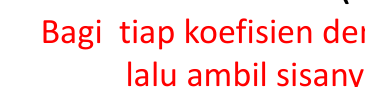
\includegraphics[width=39.90mm,height=23.76mm]{images/llm/page_056_img_01.png}%
\end{textblock*}

\newpage

% --- unit llm 57 ---
% === Halaman 57 (llm) ===

\textbf{Contoh 2}: Misalkan $a = 01010111 = x^6 + x^4 + x^2 + x + 1$ dan $b = 10000011 = x^7 + x + 1$
$a$ dan $b \in GF(2^8)$ \quad (dalam notasi Hex, $a = '57'$ dan $b = '83'$)

(i) $\begin{align*} a + b &= '57' + '83' = (x^6 + x^4 + x^2 + x + 1) + (x^7 + x + 1) \\ &= x^7 + x^6 + x^4 + x^2 + 2x + 2 \pmod{2} \\ &= x^7 + x^6 + x^4 + x^2 + 0x + 0 \\ &= x^7 + x^6 + x^4 + x^2 = 11010100 = 'D4' \end{align*}$ \vspace{5mm} $\text{\textcolor{red}{Bagi tiap koefisien dengan 2, lalu ambil sisanya}}$

Dalam representasi biner:

$\begin{array}{rl} 01010111 \\ 10000011 + \\ \hline 11010100 \end{array} \rightarrow \text{sama dengan hasil operasi XOR}$

$\therefore a + b = 11010100 = a \text{ XOR } b$

\newpage

% --- unit llm 58 ---
% === Halaman 58 (llm) ===

(ii) \begin{align*}
a \cdot b &= (x^6 + x^4 + x^2 + x + 1) \cdot (x^7 + x + 1) \\
&= x^{13} + x^7 + x^6 + x^{11} + x^5 + x^4 + x^9 + x^3 + x^2 + x^8 + x^2 + x + x^7 + x + 1 \pmod{2} \\
&= x^{13} + x^{11} + x^9 + x^8 + 2x^7 + x^6 + x^5 + x^4 + x^3 + 2x^2 + 2x + 1 \pmod{2} \\
&= x^{13} + x^{11} + x^9 + x^8 + 0x^7 + x^6 + x^5 + x^4 + x^3 + 0x^2 + 0x + 1 \\
&= x^{13} + x^{11} + x^9 + x^8 + x^6 + x^5 + x^4 + x^3 + 1
\end{align*}

Karena $m = 8$, maka hasil perkalian di atas direduksi menjadi derajat $< 8$ oleh \textit{irreducible polynomial}. Algoritma Rijndael menggunakan \textit{irreducible polynomial} $f(x) = x^8 + x^4 + x^3 + x + 1$

\[ x^{13} + x^{11} + x^9 + x^8 + x^6 + x^5 + x^4 + x^3 + 1 \pmod{f(x)} = x^7 + x^6 + 1 = 11000001 \]

$\dots a \cdot b = 11000001 = \text{'C1'}$

\newpage

% --- unit llm 59 ---
% === Halaman 59 (llm) ===

\vspace{50mm}

Jadi, \( x^{13} + x^{11} + x^9 + x^8 + x^6 + x^5 + x^4 + x^3 + 1 \pmod{f(x)} = x^7 + x^6 + 1 = 11000001 \)

% deskripsi: Proses pembagian polinomial dalam aritmatika biner (GF(2)) untuk mencari sisa pembagian (modulo).
% bbox normalisasi: [0.0600, 0.1080, 0.9400, 0.9120]
\begin{textblock*}{184.80mm}(12.60mm,32.08mm)
\noindent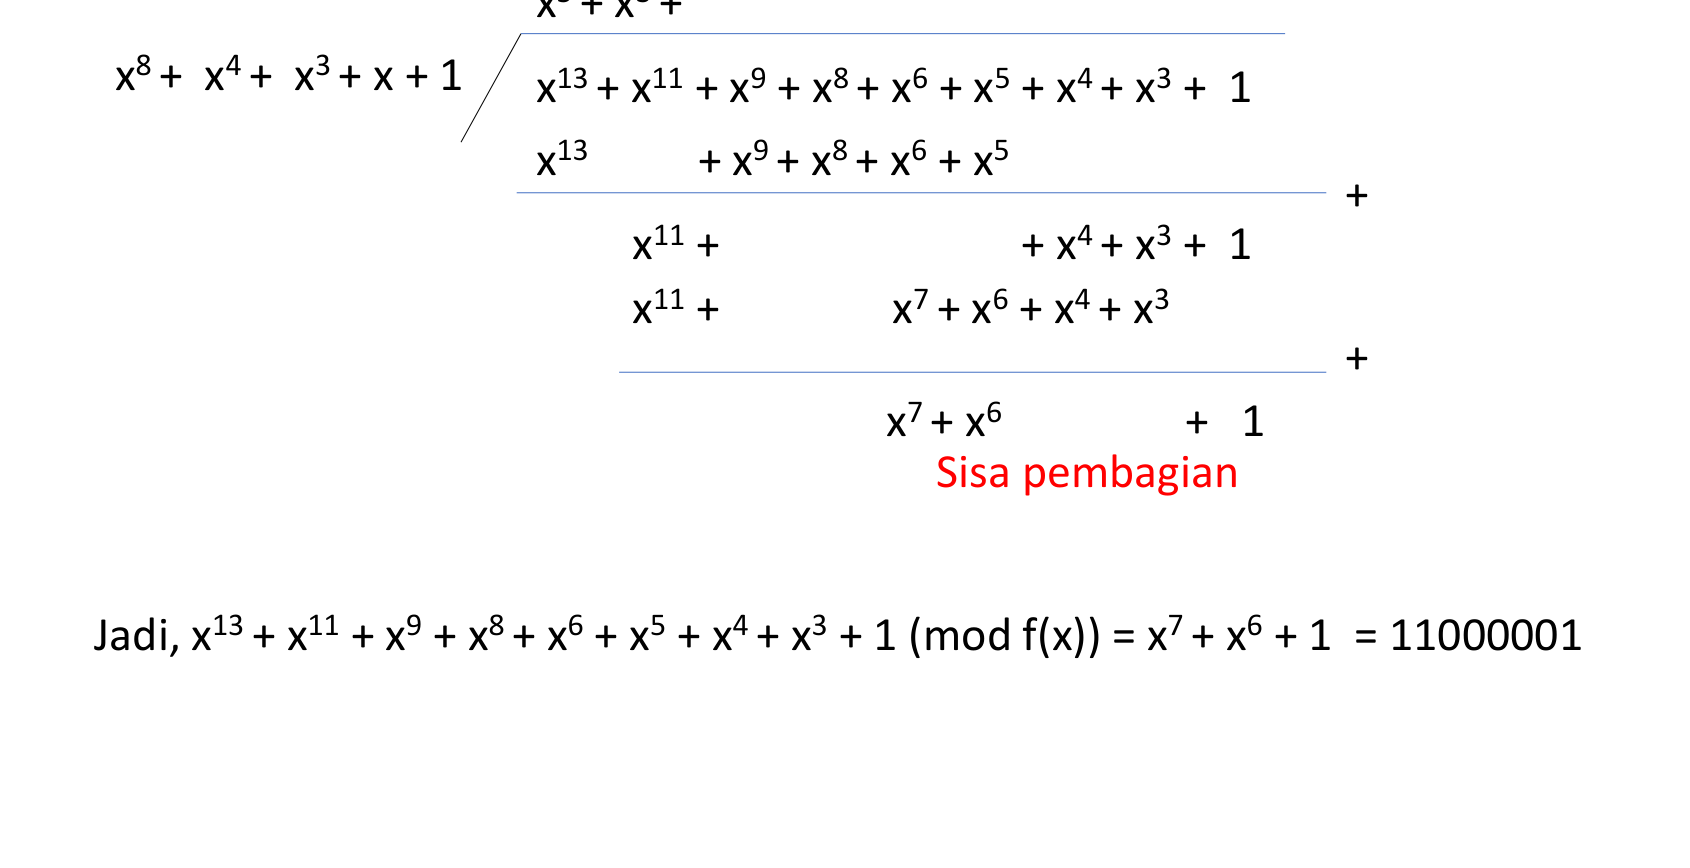
\includegraphics[width=184.80mm,height=238.79mm]{images/llm/page_059_img_01.png}%
\end{textblock*}

% bbox perkiraan otomatis: Proses pembagian polinomial dalam aritmatika biner (GF(2)) untuk mencari sisa pembagian (modulo).

\end{document}
